%% This Beamer template is based on the one found here: https://github.com/sanhacheong/stanford-beamer-presentation, and edited to be used for Stanford ARM Lab

\documentclass[10pt]{beamer}
%\mode<presentation>{}

\usepackage{media9}
\usepackage{amssymb,amsmath,amsthm,enumerate}
\usepackage{mathtools}
\usepackage[utf8]{inputenc}
\usepackage{array}
\usepackage[parfill]{parskip}
\usepackage{graphicx,animate}
\usepackage{caption}
\usepackage{subcaption}
\usepackage{bm}
\usepackage{amsfonts,amscd}
\usepackage[]{units}
\usepackage{listings}
\usepackage{multicol}
\usepackage{multirow}
\usepackage{tcolorbox}
\usepackage{physics}
\usepackage{movie15}
% Enable colored hyperlinks
\hypersetup{colorlinks=true}

% The following three lines are for crossmarks & checkmarks
\usepackage{pifont}% http://ctan.org/pkg/pifont
\newcommand{\cmark}{\ding{51}}%
\newcommand{\xmark}{\ding{55}}%

% Numbered captions of tables, pictures, etc.
\setbeamertemplate{caption}[numbered]
\usepackage{media9} 
%\usepackage[superscript,biblabel]{cite}
%\usepackage{algorithmic}
%\usepackage{algorithm2e}
\usepackage{algpseudocode}
%\usepackage[linesnumbered,ruled,vlined]{algorithm2e}
\usepackage{algorithm}
%\usepackage{algorithmic}
\usepackage{caption}
%\usepackage{xcolor}
\usepackage{array}
%\renewcommand{\thealgocf}{}

% Bibliography settings
%\usepackage[style=authoryear]{biblatex}
%\setbeamertemplate{bibliography item}{\insertbiblabel}
%
%\addbibresource{bibliography.bib}
\usepackage[natbib,backend=biber,style=ieee, sorting=ynt]{biblatex}
\bibliography{ref.bib}

% Glossary entries
\usepackage[acronym]{glossaries}

\usepackage{tikz}
\usetikzlibrary{positioning}
\usetikzlibrary{shapes,snakes}

\usepackage{graphicx}
\graphicspath{{./figures}}
\usepackage{hyperref}

\usepackage{listofitems} % for \readlist to create arrays

\colorlet{myred}{red!80!black}
\colorlet{myblue}{blue!80!black}
\colorlet{mygreen}{green!60!black}
\colorlet{myorange}{orange!70!red!60!black}
\colorlet{mydarkred}{red!30!black}
\colorlet{mydarkblue}{blue!40!black}
\colorlet{mydarkgreen}{green!30!black}
\tikzstyle{node}=[thick,circle,draw=myblue,minimum size=25,inner sep=0.5,outer sep=0.6]
\tikzstyle{node in}=[node,green!20!black,draw=mygreen!30!black,fill=mygreen!25]
\tikzstyle{node hidden}=[node,blue!20!black,draw=myblue!30!black,fill=myblue!20]
\tikzstyle{node convol}=[node,orange!20!black,draw=myorange!30!black,fill=myorange!20]
\tikzstyle{node out}=[node,red!20!black,draw=myred!30!black,fill=myred!20]
\tikzstyle{connect}=[thick,mydarkblue] %,line cap=round
\tikzstyle{connect arrow}=[-{Latex[length=4,width=3.5]},thick,mydarkblue,shorten <=0.5,shorten >=1]
\tikzset{ % node styles, numbered for easy mapping with \nstyle
  node 1/.style={node in},
  node 2/.style={node hidden},
  node 3/.style={node out},
}
\def\nstyle{int(\lay<\Nnodlen?min(2,\lay):3)} % map layer number onto 1, 2, or 3

\newacronym{ML}{ML}{machine learning}
\newacronym{HRI}{HRI}{human-robot interactions}
\newacronym{RNN}{RNN}{Recurrent Neural Network}
\newacronym{LSTM}{LSTM}{Long Short-Term Memory}


\theoremstyle{remark}
\newtheorem*{remark}{Remark}
\theoremstyle{definition}

\newcommand{\empy}[1]{{\color{darkorange}\emph{#1}}}
\newcommand{\empr}[1]{{\color{cardinalred}\emph{#1}}}
\newcommand{\examplebox}[2]{
\begin{tcolorbox}[colframe=darkcardinal,colback=boxgray,title=#1]
#2
\end{tcolorbox}}

\usetheme{Stanford} 
\def \i  {\item}
\def \ai {\item[] \quad \arrowbullet}
\newcommand \si[1]{\item[] \quad \bulletcolor{#1}}
\def \wi {\item[] \quad $\ \phantom{\Rightarrow}\ $}
\def \bi {\begin{itemize}\item}
\def \ei {\end{itemize}}
\def \be {\begin{equation*}}
\def \ee {\end{equation*}}
\def \bie {$\displaystyle{}
\def \eie {{\ }$}}
\def \bsie {\small$\displaystyle{}
\def \esie {{\ }$}\normalsize\selectfont}
\def \bse {\small\begin{equation*}}
\def \ese {\end{equation*}\normalsize}
\def \bfe {\footnotesize\begin{equation*}}
\def \efe {\end{equation*}\normalsize}
\renewcommand \le[1] {\\ \medskip \lefteqn{\hspace{1cm}#1} \medskip}
\def \bex {\begin{example}}
\def \eex {\end{example}}
\def \bfig {\begin{figure}}
\def \efig {\end{figure}}
\def \btheo {\begin{theorem}}
\def \etheo {\end{theorem}}
\def \bc {\begin{columns}}
\def \ec {\end{columns}}
\def \btab {\begin{tabbing}}
\def \etab {\end{tabbing}\svneg\svneg}
\newcommand \col[1]{\column{#1\linewidth}}
\def\vneg  {\vspace{-5mm}}
\def\lvneg {\vspace{-10mm}}
\def\svneg {\vspace{-2mm}}
\def\tvneg {\vspace{-1mm}}
\def\vpos  {\vspace{5mm}}
\def\lvpos {\vspace{10mm}}
\def\svpos {\vspace{2mm}}
\def\tvpos {\vspace{1mm}}
\def\hneg  {\hspace{-5mm}}
\def\lhneg {\hspace{-10mm}}
\def\shneg {\hspace{-2mm}}
\def\thneg {\hspace{-1mm}}
\def\hpos  {\hspace{5mm}}
\def\lhpos {\hspace{10mm}}
\def\shpos {\hspace{2mm}}

\logo{
\includegraphics[height=0.5in]{logos/HUS-name.jpg}}

\makeatletter
\let\@@magyar@captionfix\relax
\makeatother

\title[Backpropagation For Training Deep Neural Networks]{Backpropagation \\ For Training Deep Neural Networks}


\begin{document}

\nocite{*}

\author[Chi Thanh Nguyen - Duc Thinh Nguyen]{
	\begin{tabular}{c} 
	\Large
	Chi Thanh Nguyen \\
    \footnotesize \href{mailto:nguyenchithanh\_sdh21@hus.edu.vn}{nguyenchithanh\_sdh21@hus.edu.vn} \\
	\Large
    Duc Thinh Nguyen \\
     \footnotesize \href{mailto:nguyenducthinh\_sdh21@hus.edu.vn}{nguyenducthinh\_sdh21@hus.edu.vn}
\end{tabular}
\vspace{-4ex}}

\institute{
	\vskip 5pt
	\begin{figure}
		\centering
		\begin{subfigure}[t]{0.5\textwidth}
			\centering
			
\includegraphics[height=0.75in]{logos/HUS-logo.jpg}
		\end{subfigure}%
		~ 
		\begin{subfigure}[t]{0.5\textwidth}
			\centering
			
\includegraphics[height=0.75in]{logos/MIM-logo.png}
		\end{subfigure}
	\end{figure}
	\vskip 10pt	
	Vietnam National University \\
	Hanoi University of Science\\
	Faculty of Mathematics, Mechanics and Informatics
	\vskip 3pt
}

% \date{June 15, 2020}
%\date{\today}

\begin{noheadline}
\begin{frame} \maketitle \end{frame}
\end{noheadline}

\setbeamertemplate{itemize items}[default]
\setbeamertemplate{itemize subitem}[circle]

\begin{frame}{Content}

\begin{enumerate}
	\item Introduction
 	\item Notations
	\item Formulations
	\item Experiment
 	\item Conclusion
\end{enumerate}

\end{frame}

\begin{frame}[allowframebreaks]{Introduction}
	\begin{figure}
		\centering
		\resizebox{5cm}{!}{%
		\begin{tikzpicture}
			\node [circle, draw=black!60, fill=blue!30, minimum size=10mm] (bias) at (0, 5) {1};
			
			\node[circle, draw=black!60, fill=cyan!60, minimum size=12mm] (x_1) at (0, 3) {$x_1$};
			
			\node[circle, draw=black!60, fill=cyan!60, minimum size=12mm] (x_2) at (0, 1) {$x_2$};
			
			\path (x_2) --++ (0, -3) node[midway,scale=5] {$\vdots$};
			
			\node[circle, draw=black!60, fill=cyan!60, minimum size=12mm] (x_d) at (0, -4) {$x_d$};
			
			\node[circle split, draw=black!60, rotate=90, fill=white, minimum size = 30mm] (z) at (6, 0){\rotatebox{-90}{$z=\displaystyle\sum$} \nodepart{lower} \rotatebox{-90}{$a=\mathbf{f}(z)$}};
			
			\draw[->] (bias) -- (z) node[midway,above] {$b$};
			\draw[->] (x_1) -- (z) node[midway,above] {$w_1$};
			\draw[->] (x_2) -- (z) node[midway,above] {$w_2$};
			\draw[->] (x_d) -- (z) node[midway,below] {$w_d$};
			
			\node at (10, 0) {$\begin{cases}z=\displaystyle\sum_{i=1}^d w_i x_i + b \\ a = \mathbf{f}(z) \end{cases}$};
		\end{tikzpicture}
		}
		\caption{A neural network unit}
		\label{fig:Single neuron model}
	\end{figure}

	\begin{itemize}
		\item A neural network unit is a primitive neural network that consists of only the input layer, and an output layer with only one output.
  		\item A neural network unit computes a non-linear weighted combination of its inputs. 
	\end{itemize}

	Some popular activation functions:

	%\begin{table} [h!]
	%	\centering
	%	\begin{tabular}{ || c | c  || }
	%	\hline
	%	Activation Function & Formula \\ [0.5 ex]
	%	\hline \hline
	%	ReLU & $\bold{f}(z) = \max(0, z)$ \\ \hline
	%	Sigmoid & $\bold{f}(z) = \dfrac{1}{1 + e^{-z}}$ \\ \hline
	%	Tanh & $\bold{f}(z) = \dfrac{e^z - e^{-z}}{e^z + e^{-z}}$ \\ \hline
	%	Leaky ReLU & $\bold{f}(z)=\max(z, \alpha z) \text{ for } 0 < \alpha < 1 $ \\ \hline
	%	17 & 18 \\ [1ex]
	%	\hline
	%	\end{tabular}
	%	\caption{Popular activation functions}
	%	\end{table}
	\begin{itemize}
		\item ReLU:
		\begin{equation*}
			\bold{f}(z) = \max(0, z)
		\end{equation*}
		\item Sigmoid:
		\begin{equation*}
			\bold{f}(z) = \dfrac{1}{1 + e^{-z}}
		\end{equation*}
		\item Tanh:
		\begin{equation*}
			\bold{f}(z) = \dfrac{e^z - e^{-z}}{e^z + e^{-z}}
		\end{equation*}
		\item Leaky ReLU:
		\begin{equation*}
			\bold{f}(z)=\max(z, \alpha z) \text{ for } 0 < \alpha < 1
		\end{equation*}
		\item ELU:
		\begin{equation*}
			\bold{f}(z) = \begin{cases} z \text{ for } z \geq 0 \\ \alpha (e^z - 1) \text{ for } z < 0 \end{cases}
		\end{equation*}
		\item GELU:
		\begin{equation*}
			\bold{f}(z)=0.5 z \Bigg( 1 + \dfrac{2}{\sqrt{\pi}} \int_0^{\frac{z}{\sqrt{2}}} e^{-x^2}dx \Bigg)
		\end{equation*}
		\item Swish:
		\begin{equation*}
			\bold{f}(z) = \dfrac{z}{1 + e^{-z}}
		\end{equation*}
		\item Softplus:
		\begin{equation*}
			\bold{f}(z) = \ln(1 + e^z)
		\end{equation*}
	\end{itemize}

	\begin{figure}
		\centering
		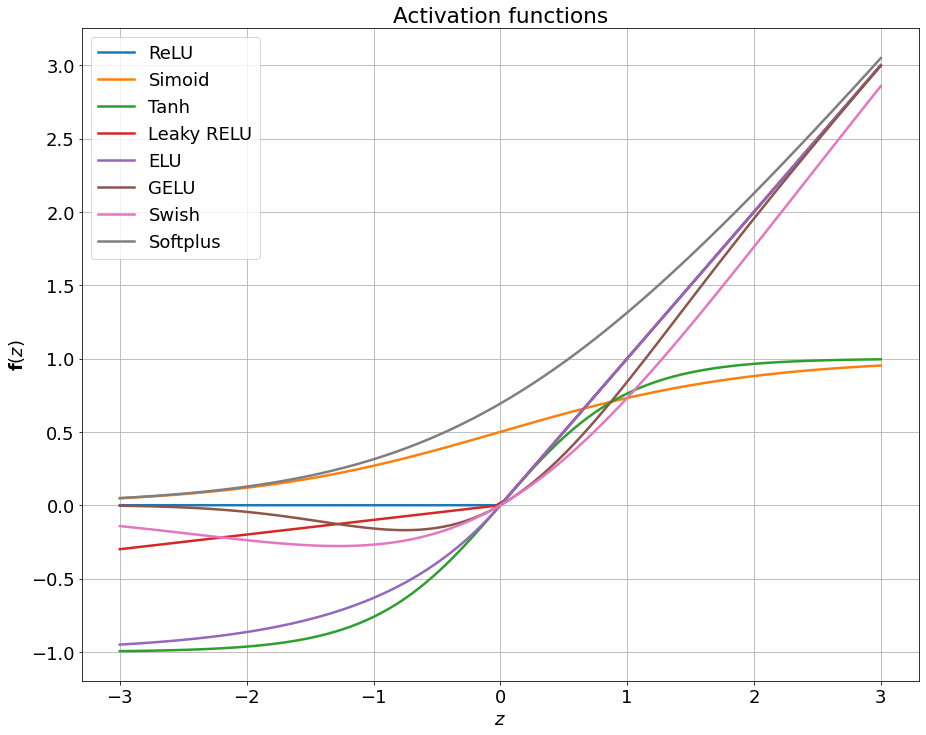
\includegraphics[width=9cm]{activation_functions.png}
		\caption{Activation functions}
	\end{figure}

	\begin{figure}
		\centering
		\resizebox{8cm}{!}{
			\begin{tikzpicture}[x=2.2cm,y=1.4cm]
				\message{^^JNeural network, shifted}
				\readlist\Nnod{4,5,5,5,3} % array of number of nodes per layer
				\readlist\Nstr{d^{(0)}, d^{(1)}, d^{(2)}, d^{(3)}, d^{(4)}} % array of string number of nodes per layer
				\readlist\Cstr{\strut x,a^{(\prev)},a^{(\prev)},a^{(\prev)},\hat{y}} % array of coefficient symbol per layer
				\def\yshift{0.5} % shift last node for dots
				
				\message{^^J  Layer}
				\foreachitem \N \in \Nnod{ % loop over layers
				  \def\lay{\Ncnt} % alias of index of current layer
				  \pgfmathsetmacro\prev{int(\Ncnt-1)} % number of previous layer
				  \message{\lay,}
				  \foreach \i [evaluate={\c=int(\i==\N); \y=\N/2-\i-\c*\yshift;
							   \index=(\i<\N?int(\i):"\Nstr[\lay]");
							   \x=\lay; \n=\nstyle;}] in {1,...,\N}{ % loop over nodes
					% NODES
					\node[node \n] (N\lay-\i) at (\x,\y) {$\Cstr[\lay]_{\index}$};
					
					% CONNECTIONS
					\ifnum\lay>1 % connect to previous layer
					  \foreach \j in {1,...,\Nnod[\prev]}{ % loop over nodes in previous layer
						\draw[connect,white,line width=1.2] (N\prev-\j) -- (N\lay-\i);
						\draw[connect] (N\prev-\j) -- (N\lay-\i);
						%\draw[connect] (N\prev-\j.0) -- (N\lay-\i.180); % connect to left
					  }
					\fi % else: nothing to connect first layer
					
				  }
				  \path (N\lay-\N) --++ (0,1+\yshift) node[midway,scale=1.5] {$\vdots$};
				}
				
				% LABELS
				\node[above=0.5cm,align=center,mygreen!60!black] at (N1-1.90) {input\\[-0.2em]layer};
				\node[above=0.5cm,align=center,myblue!60!black] at (N3-1.90) {hidden layers};
				\node[above=0.5cm,align=center,myred!60!black] at (N\Nnodlen-1.90) {output\\[-0.2em]layer};
				
			\end{tikzpicture}
		}
		\caption{A neural network with 3 hidden layers}
	\end{figure}

\end{frame}

\begin{frame}[allowframebreaks]{Notations}
	\begin{itemize}
		\item $a$: A scalar
  		\item $\bold{a}$: A vector
    	\item $\bold{W}$: A matrix
     	\item $\bold{W}_{i,:}$: Row $i$ of matrix $\bold{W}$
      	\item $\bold{W}_{:,j}$ or $\bold{w}_j$: Column $j$ of matrix $\bold{W}$
       	\item $\bold{W^{(l)}}$: Weights from (l-1)-th layer to l-th layer
        \item $\bold{b}^{(l)}$: Biases from (l-1)-th layer to l-th layer
        \item $w_{ij}^{(l)}$: The weight from i-th neuron of (l-1)-th layer to jth neuron lth layer
        \item $z_{i}^{(l)}$: The pre-activated output of neuron i-th of l-th layer
        \item $a_{i}^{(l)}$: The activated output of neuron i-th of l-th layer
        \item $d^{(l)}$: The number of neuron (dimension) of l-th layer
        \item $\bold{z}^{(l)}$: The pre-activated output vector of l-th layer. $\bold{z}^{(l)} = \begin{bmatrix} z_1^{(l)} & z_2^{(l)} & \dots & z_{d^{(l)}}^{(l)}\end{bmatrix}^T$
        \item $\bold{a}^{(l)}$: The activated output vector of l-th layer. $\bold{a}^{(l)} = \begin{bmatrix} a_1^{(l)} & a_2^{(l)} &\dots & a_{d^{(l)}}^{(l)}\end{bmatrix}^T$
        \item $\mathcal{L}$: The loss function
        \item $\odot$: An element-wise product of two vectors
        \item $\bold{x}=\bold{a}^{(0)}$: An input of neural network
	\end{itemize}

\end{frame}

\begin{frame}[allowframebreaks]{Formulations}
	\begin{algorithm}[H]
		\caption{Training neural networks}
		\begin{algorithmic}[1]
			\State{Initialize neural network weights $\bold{W}$ randomly}
			\While{not converged}
				\State{Get training samples} (data loading)
				\State{Calculate neural network outputs and the loss function $\mathcal{L}$} (forward pass)
				\State{Calculate partial derivatives of the loss funtion with respect to $\bold{W}$}
				\State{Update neural network weights: \begin{equation*}
					\bold{W} \leftarrow \bold{W} - \alpha  \dfrac{\partial \mathcal{L}}{\partial \bold{W}}
				\end{equation*}}
			\EndWhile
		\end{algorithmic}
	\end{algorithm}

	\begin{itemize}
		\item Problem: But how do we calculate $\dfrac{\partial \mathcal{L}}{\partial \bold{W}}$?
  		\item We can calculate $\dfrac{\partial \mathcal{L}}{\partial \bold{W}}$ by a technique called Backpropagation
	\end{itemize}

	\begin{itemize}
		\item Backpropagation: Partial derivatives of loss function with respect to outputs of a layer computed by partial derivatives of loss function with respect to outputs of its successive layer
  		\item One training step can decompose into 3 stages:
		\begin{itemize}
			\item Foward pass: Compute output of deep neural network and loss function
   			\item Backward pass (Backpropagation): Calculate gradient of loss function with respect to weights of layers. Start from top (output) to first (input) layer
      		\item Update: Update neural network weights
		\end{itemize}
	\end{itemize}
	\framebreak
	\begin{itemize}
		\item $\bold{W}^{(l)}$: weights of l-th layer
    	\begin{equation*}
			\bold{W}^{(l)}=\begin{bmatrix} w_{11}^{(l)} & w_{12}^{(l)} & w_{13}^{(l)} & \dots & w_{1d^{(l)}}^{(l)} \\ w_{21}^{(l)} & w_{22}^{(l)} & w_{23}^{(l)} & \dots & w_{2d^{(l)}}^{(l)} \\ \vdots & \thickspace & \thickspace & \thickspace & \vdots \\ w_{d^{(l-1)}1}^{(l)} & w_{d^{(l-1)}2}^{(l)} & w_{d^{(l-1)}3}^{(l)} & \dots & w_{d^{(l-1)}d^{(l)}}^{(l)}\end{bmatrix} \in \mathbb{R}^{d^{(l-1)} \times d^{(l)}}
		\end{equation*}
		\item $\bold{b}^{(l)}$: biases of l-th layer
		\begin{equation*}
			\bold{b}^{(l)}=\begin{bmatrix} b_1^{(l)} \\  b_2^{(l)} \\ \vdots \\ b_{d^{(l)}}^{(l)} \end{bmatrix}
		\end{equation*}
		\begin{figure}
			\centering
			\resizebox{9.5cm}{!}{
				\begin{tikzpicture}

					\tikzstyle{every node}=[font=\Large]
					
					\node [circle, draw=black!60, fill=blue!30, minimum size=8mm] (bias_l_minus_1) at (0, 0) {1};
					
					\node[circle, draw=black!60, fill=cyan!60, minimum size=10mm, label={[label distance=0.1cm]-120:$z_1^{(l-1)}$}, label={[label distance=0.1cm]-60:$a_1^{(l-1)}$}] (neuron_1_l_minus_1) at (0, -2.5) {};
					
					\node[circle, draw=black!60, fill=cyan!60, minimum size=10mm, label={[label distance=0.1cm]-120:$z_i^{(l-1)}$}, label={[label distance=0.1cm]-60:$a_i^{(l-1)}$}] (neuron_i_l_minus_1) at (0, -7.5) {};
					
					\node[circle, draw=black!60, fill=cyan!60, minimum size=10mm, label={[label distance=0.1cm]-120:$z_{d^{(l-1)}}^{(l-1)}$}, label={[label distance=0.1cm]-60:$a_{d^{(l-1)}}^{(l-1)}$}] (neuron_d_l_minus_1) at (0, -12.5) {};
					
					\path (neuron_1_l_minus_1) --++ (0, -4) node[midway,scale=5] {$\vdots$};
					\path (neuron_i_l_minus_1) --++ (0, -4) node[midway,scale=5] {$\vdots$};
					
					\node [circle, draw=black!60, fill=blue!30, minimum size=8mm] (bias_l) at (6, 0) {1};
					
					
					\node[circle, draw=black!60, fill=cyan!60, minimum size=10mm, label={[label distance=0.1cm]-120:$z_1^{(l)}$}, label={[label distance=0.1cm]-60:$a_1^{(l)}$}] (neuron_1_l) at (6, -2.5) {};
					
					\node[circle, draw=black!60, fill=cyan!60, minimum size=10mm, label={[label distance=0.1cm]-120:$z_2^{(l)}$}, label={[label distance=0.1cm]-60:$a_2^{(l)}$}] (neuron_2_l) at (6, -5) {};
					
					\node[circle, draw=black!60, fill=cyan!60, minimum size=10mm, label={[label distance=0.1cm]-120:$z_j^{(l)}$}, label={[label distance=0.1cm]-60:$a_j^{(l)}$}] (neuron_j_l) at (6, -10) {};
					
					\node[circle, draw=black!60, fill=cyan!60, minimum size=10mm, label={[label distance=0.1cm]-120:$z_{d^{(l)}}^{(l)}$}, label={[label distance=0.1cm]-60:$a_{d^{(l)}}^{(l)}$}] (neuron_d_l) at (6, -15) {};
					
					\path (neuron_2_l) --++ (0, -4.5) node[midway,scale=5] {$\vdots$};
					\path (neuron_j_l) --++ (0, -4.5) node[midway,scale=5] {$\vdots$};
					
					\draw[->] (bias_l_minus_1) -- (neuron_1_l) node[midway,above] {$b_1^{(l)}$};
					\draw[->, dotted] (bias_l_minus_1) -- (neuron_2_l);
					\draw[->, dotted] (bias_l_minus_1) -- (neuron_j_l);
					\draw[->, dotted] (bias_l_minus_1) -- (neuron_d_l);
					
					\draw[->] (neuron_1_l_minus_1) -- (neuron_1_l) node[midway,above] {$w_{11}^{(l)}$};
					\draw[->, dotted] (neuron_1_l_minus_1) -- (neuron_2_l);
					\draw[->, dotted] (neuron_1_l_minus_1) -- (neuron_j_l);
					\draw[->, dotted] (neuron_1_l_minus_1) -- (neuron_d_l);
					
					\draw[->] (neuron_i_l_minus_1) -- (neuron_1_l) node[midway,above=0.2cm] {$w_{i1}^{(l)}$};
					\draw[->] (neuron_i_l_minus_1) -- (neuron_2_l) node[midway,above=0.2cm] {$w_{i2}^{(l)}$};
					\draw[->] (neuron_i_l_minus_1) -- (neuron_j_l) node[midway,above] {$w_{ij}^{(l)}$};
					\draw[->] (neuron_i_l_minus_1) -- (neuron_d_l) node[midway,below=0.2cm] {$w_{id^{(l)}}^{(l)}$};
					
					\draw[->] (neuron_d_l_minus_1) -- (neuron_1_l) node[midway,above] {$w_{d^{(l-1)}1}^{(l)}$};
					\draw[->, dotted] (neuron_d_l_minus_1) -- (neuron_2_l);
					\draw[->, dotted] (neuron_d_l_minus_1) -- (neuron_j_l);
					\draw[->, dotted] (neuron_d_l_minus_1) -- (neuron_d_l);

					\node[above=1,align=center] at (bias_l_minus_1.90) {(l-1)-th layer};
					\node[above=1,align=center] at (bias_l.90) {l-th layer};
					
					\node at (-10, -5) {$\begin{cases} \bold{W}^{(l)}=\begin{bmatrix} w_{11}^{(l)} & w_{12}^{(l)} & w_{13}^{(l)} & \dots & w_{1d^{(l)}}^{(l)} \\ w_{21}^{(l)} & w_{22}^{(l)} & w_{23}^{(l)} & \dots & w_{2d^{(l)}}^{(l)} \\ \vdots & \thickspace & \thickspace & \thickspace & \vdots \\ w_{d^{(l-1)}1}^{(l)} & w_{d^{(l-1)}2}^{(l)} & w_{d^{(l-1)}3}^{(l)} & \dots & w_{d^{(l-1)}d^{(l)}}^{(l)}\end{bmatrix} \in \mathbb{R}^{d^{(l-1)} \times d^{(l)}} \\ \bold{b}^{(l)}=\begin{bmatrix} b_1^{(l)} \\  b_2^{(l)} \\ \vdots \\ b_{d^{(l)}}^{(l)} \end{bmatrix} \in \mathbb{R}^{d^{(l)}} \end{cases}$};
				\end{tikzpicture}
			}
			\caption{Visualization of two successive layers}
		\end{figure}
		\item The pre-activated output of neuron i of l-th layer:
		\begin{equation}
			z_j^{(l)}=\sum_{i=1}^{d^{(l-1)}}w_{ij}^{(l)}a_i^{(l-1)}+b_j^{(l)}=\Big(\bold{W}_{:,j}^{(l)}\Big)^T \bold{a}^{(l-1)} + b_j^{(l)}
		\end{equation}
		\item The activated output of neuron i of l-th layer:
		\begin{equation}
			a_j^{(l)} = \bold{f}(z_j^{(l)})
		\end{equation}
		\item The pre-activated output in matrix form:
		\begin{equation}
			\bold{z}^{(l)}=\Big(\bold{W}^{(l)}\Big)^T\bold{a}^{(l-1)} + \bold{b}^{(l)}, l=1, \dots, L
		\end{equation}
		\item Activated outputs in matrix form:
		\begin{equation}
			\bold{a}^{(l)}=\bold{f}(\bold{z}^{(l)}), l=1, \dots, L
		\end{equation}
		\begin{figure}
			\centering
			\resizebox{8.0cm}{!}{
				\begin{tikzpicture}
	
					\tikzstyle{every node}=[font=\Large]
					\node [circle, draw=black!60, fill=blue!30, minimum size=8mm] (bias_l_minus_1) at (0, 0) {1};
					
					\node[circle, draw=black!60, fill=cyan!60, minimum size=10mm, label={[label distance=0.1cm]-120:$z_1^{(l-1)}$}, label={[label distance=0.1cm]-60:$a_1^{(l-1)}$}] (neuron_1_l_minus_1) at (0, -2.5) {};
					
					\node[circle, draw=black!60, fill=cyan!60, minimum size=10mm, label={[label distance=0.1cm]-120:$z_i^{(l-1)}$}, label={[label distance=0.1cm]-60:$a_i^{(l-1)}$}] (neuron_i_l_minus_1) at (0, -7.5) {};
					
					\node[circle, draw=black!60, fill=cyan!60, minimum size=10mm, label={[label distance=0.1cm]-120:$z_{d^{(l-1)}}^{(l-1)}$}, label={[label distance=0.1cm]-60:$a_{d^{(l-1)}}^{(l-1)}$}] (neuron_d_l_minus_1) at (0, -12.5) {};
					
					\path (neuron_1_l_minus_1) --++ (0, -4) node[midway,scale=5] {$\vdots$};
					\path (neuron_i_l_minus_1) --++ (0, -4) node[midway,scale=5] {$\vdots$};
					
					\node [circle, draw=black!60, fill=blue!30, minimum size=8mm] (bias_l) at (6, 0) {1};
					
					
					\node[circle, draw=black!60, fill=cyan!60, minimum size=10mm, label={[label distance=0.1cm]-120:$z_1^{(l)}$}, label={[label distance=0.1cm]-60:$a_1^{(l)}$}] (neuron_1_l) at (6, -2.5) {};
					
					\node[circle, draw=black!60, fill=cyan!60, minimum size=10mm, label={[label distance=0.1cm]-120:$z_j^{(l)}$}, label={[label distance=0.1cm]-60:$a_j^{(l)}$}] (neuron_j_l) at (6, -9) {};
					
					\node[circle, draw=black!60, fill=cyan!60, minimum size=10mm, label={[label distance=0.1cm]-120:$z_{d^{(l)}}^{(l)}$}, label={[label distance=0.1cm]-60:$a_{d^{(l)}}^{(l)}$}] (neuron_d_l) at (6, -14) {};
					
					\path (neuron_1_l) --++ (0, -4.5) node[midway,scale=5] {$\vdots$};
					\path (neuron_j_l) --++ (0, -4.5) node[midway,scale=5] {$\vdots$};
					
					\node [circle, draw=black!60, fill=blue!30, minimum size=8mm] (bias_l_plus_1) at (12, 0) {1};
					
					
					\node[circle, draw=black!60, fill=cyan!60, minimum size=10mm, label={[label distance=0.1cm]-120:$z_1^{(l+1)}$}, label={[label distance=0.1cm]-60:$a_1^{(l+1)}$}] (neuron_1_l_plus_1) at (12, -2.5) {};
					
					\node[circle, draw=black!60, fill=cyan!60, minimum size=10mm, label={[label distance=0.1cm]-120:$z_k^{(l)}$}, label={[label distance=0.1cm]-60:$a_k^{(l)}$}] (neuron_k_l_plus_1) at (12, -7) {};
					
					\node[circle, draw=black!60, fill=cyan!60, minimum size=10mm, label={[label distance=0.1cm]-120:$z_{d^{(l+1)}}^{(l+1)}$}, label={[label distance=0.1cm]-60:$a_{d^{(l+1)}}^{(l+1)}$}] (neuron_d_l_plus_1) at (12, -11.5) {};
					
					\path (neuron_1_l_plus_1) --++ (0, -3.0) node[midway,scale=5] {$\vdots$};
					\path (neuron_k_l_plus_1) --++ (0, -3.0) node[midway,scale=5] {$\vdots$};
					
					\draw[->] (bias_l_minus_1) -- (neuron_1_l) node[midway,above] {$b_1^{(l)}$};
					\draw[->, dotted] (bias_l_minus_1) -- (neuron_j_l);
					\draw[->, dotted] (bias_l_minus_1) -- (neuron_d_l);
					
					\draw[->, dotted] (neuron_1_l_minus_1) -- (neuron_1_l);
					\draw[->, dotted] (neuron_1_l_minus_1) -- (neuron_j_l);
					\draw[->, dotted] (neuron_1_l_minus_1) -- (neuron_d_l);
					
					\draw[->] (neuron_i_l_minus_1) -- (neuron_1_l) node[midway,above=0.2cm] {$w_{i1}^{(l)}$};
					\draw[->] (neuron_i_l_minus_1) -- (neuron_j_l) node[midway,above] {$w_{ij}^{(l)}$};
					\draw[->] (neuron_i_l_minus_1) -- (neuron_d_l) node[midway,below=0.2cm] {$w_{id^{(l)}}^{(l)}$};
					
					\draw[->, dotted] (neuron_d_l_minus_1) -- (neuron_1_l);
					\draw[->, dotted] (neuron_d_l_minus_1) -- (neuron_j_l);
					\draw[->, dotted] (neuron_d_l_minus_1) -- (neuron_d_l);
					
					\draw[->, dotted] (bias_l) -- (neuron_1_l_plus_1);
					\draw[->] (bias_l) -- (neuron_k_l_plus_1) node[midway, above=0.5cm] {$b_{k}^{(l+1)}$};
					\draw[->, dotted] (bias_l) -- (neuron_d_l_plus_1);
					
					\draw[->, dotted] (neuron_1_l) -- (neuron_1_l_plus_1);
					\draw[->] (neuron_1_l) -- (neuron_k_l_plus_1) node[midway, below=0.25cm] {$w_{1k}^{(l+1)}$};
					\draw[->, dotted] (neuron_1_l) -- (neuron_d_l_plus_1);
					
					\draw[->, dotted] (neuron_j_l) -- (neuron_1_l_plus_1);
					\draw[->] (neuron_j_l) -- (neuron_k_l_plus_1) node[midway, above=0.25cm] {$w_{jk}^{(l+1)}$};
					\draw[->, dotted] (neuron_j_l) -- (neuron_d_l_plus_1);
					
					\draw[->, dotted] (neuron_d_l) -- (neuron_1_l_plus_1);
					\draw[->] (neuron_d_l) -- (neuron_k_l_plus_1) node[midway, above=0.5cm] {$w_{d^{(l)}k}^{(l+1)}$};
					\draw[->, dotted] (neuron_d_l) -- (neuron_d_l_plus_1);
					
					\node[above=1,align=center] at (bias_l_minus_1.90) {(l-1)-th layer};
					\node[above=1,align=center] at (bias_l.90) {l-th layer};
					\node[above=1,align=center] at (bias_l_plus_1.90) {(l+1)-th layer};
					
					\node[below=2, align=center] at (neuron_d_l_minus_1.-90) {$\mathbf{z}^{(l-1)}-\mathbf{a}^{(l-1)}$};
					
					\node[below=2, align=center] at (neuron_d_l.-90) {$\mathbf{z}^{(l)}-\mathbf{a}^{(l)}$};
					
					\node[below=2, align=center] at (neuron_d_l_plus_1.-90) {$\mathbf{z}^{(l+1)}-\mathbf{a}^{(l+1)}$};
					
					\node at (-5, 0) {$\begin{cases}\mathbf{W}^{(l)} \in \mathbb{R}^{d^{(l)}\times d^{(l+1)}} \\ \mathbf{b}^{(l)} \in \mathbb{R}^{d^{(l)}} \end{cases}$};
					
					\node at (-5, -3) {$\begin{aligned}z_j^{(l)}&=\displaystyle\sum_{i=1}^{d^{(l-1)}}w_{ij}^{(l)}a_i^{(l-1)}+b_j^{(l)}\\&=\Big(\bold{W}_{:,j}^{(l)}\Big)^T \bold{a}^{(l-1)} + b_j^{(l)}\end{aligned}$};
					
					\node at (-5, -5) {$\bold{z}^{(l)}=\Big(\bold{W}^{(l)}\Big)^T\bold{a}^{(l-1)} + \bold{b}^{(l)}$};
					
					\node at (-5, -8) {$\begin{aligned} a_j^{(l)} &= \mathbf{f} \big( z_i^{(l)} \big)\\&=\mathbf{f} \Big(\displaystyle\sum_{i=1}^{d^{(l-1)}}w_{ij}^{(l)}a_i^{(l-1)}+b_j^{(l)} \Big) \\&= \mathbf{f} \Big\lbrack \Big(\bold{W}_{:,j}^{(l)}\Big)^T \bold{a}^{(l-1)} + b_j^{(l)} \Big\rbrack \end{aligned}$};
					
					\node at (-5, -12) {$\begin{aligned} \mathbf{a}^{(l)}&=\mathbf{f} \Big( \mathbf{z}^{(l)} \Big)\\&=\mathbf{f} \Big\lbrack\Big(\bold{W}^{(l)}\Big)^T\bold{a}^{(l-1)} + \bold{b}^{(l)} \Big\rbrack \end{aligned}$};
				\end{tikzpicture}
			}
			\caption{Visualization of three layers}
		\end{figure}
		\item The loss function:
		\begin{equation}
			\mathcal{L} = \ell\Big(\bold{a}^{(L)}, \bold{y} \Big)
		\end{equation}
	\end{itemize}

	We need to calculate partial derivatives of $\mathcal{L}$ with respect to all $\bold{W}^{(l)}$ and $\bold{b}^{(l)}, l=1, \dots, L$

	\begin{equation}
		\dfrac{\partial \mathcal{L}}{w_{ij}^{(l)}}=\dfrac{\partial \mathcal{L}}{\partial z_{j}^{(l)}}\dfrac{\partial z_j^{(l)}}{w_{ij}^{(l)}}=\dfrac{\partial \mathcal{L}}{\partial z_{j}^{(l)}}a_i^{(l-1)}
	\end{equation}

	\begin{equation}
		\dfrac{\partial \mathcal{L}}{\partial b_j^{(l)}}=\dfrac{\partial \mathcal{L}}{\partial z_{j}^{(l)}}\dfrac{\partial z_j^{(l)}}{\partial b_j^{(l)}}=\dfrac{\partial \mathcal{L}}{\partial z_{j}^{(l)}}
	\end{equation}

	We set:
	\begin{equation}
		\dfrac{\partial \mathcal{L}}{\partial z_{j}^{(l)}}:=e_j^{(l)}
	\end{equation}

	At the output layer ($L$-th layer):

	\begin{equation}
		\begin{aligned}
			\dfrac{\partial \mathcal{L}}{w_{ij}^{(L)}}&=\dfrac{\partial \mathcal{L}}{\partial z_{j}^{(L)}}\dfrac{\partial z_j^{(L)}}{w_{ij}^{(L)}}\\&=\dfrac{\partial \mathcal{L}}{\partial z_{j}^{(L)}}a_i^{(L-1)}\\&=\dfrac{\partial\mathcal{L}}{\partial a_j^{(L)}}\dfrac{\partial a_j^{(L)}}{\partial z_j^{(L)}}a_i^{(L-1)}\\&=\dfrac{\partial\mathcal{L}}{\partial a_j^{(L)}}\bold{f}^{\prime}\Big(z_j^{(L)}\Big)a_i^{(L-1)}
		\end{aligned}
	\end{equation}

	\begin{equation}
		\begin{aligned}
			\bold{e}^{(L)}&=\begin{bmatrix} \dfrac{\partial\mathcal{L}}{\partial z_1^{(L)}} & \dfrac{\partial\mathcal{L}}{\partial z_2^{(L)}} & \dots & \dfrac{\partial\mathcal{L}}{\partial z_{d^{(L)}}^{(L)}} \end{bmatrix}^T\\&=\begin{bmatrix} \dfrac{\partial\mathcal{L}}{\partial a_1^{(L)}}\dfrac{\partial a_1^{(L)}}{\partial z_1^{(L)}} & \dfrac{\partial\mathcal{L}}{\partial a_2^{(L)}}\dfrac{\partial a_2^{(L)}}{\partial z_2^{(L)}} & \dots & \dfrac{\partial\mathcal{L}}{\partial a_{d^{(L)}}^{(L)}}\dfrac{\partial a_{d^{(L)}}^{(L)}}{\partial z_{d^{(L)}}^{(L)}} \end{bmatrix}^T\\&=\begin{bmatrix} \dfrac{\partial\mathcal{L}}{\partial a_1^{(L)}}\bold{f}^{\prime}\Big(z_1^{(L)}\Big) & \dfrac{\partial\mathcal{L}}{\partial a_2^{(L)}}\bold{f}^{\prime}\Big(z_2^{(L)}\Big) & \dots & \dfrac{\partial\mathcal{L}}{\partial a_{d^{(L)}}^{(L)}}\bold{f}^{\prime}\Big(z_{d^{(L)}}^{(L)}\Big) \end{bmatrix}^T\\&=\dfrac{\partial \mathcal{L}}{\partial \bold{a}^{(L)}} \odot \bold{f}^{\prime}(\bold{z}^{(L)})
		\end{aligned}
	\end{equation}

	\begin{equation}
		\Rightarrow \begin{cases}\dfrac{\partial \mathcal{L}}{\partial \bold{W}^{(L)}}=\bold{a}^{(L-1)}\Big(\bold{e}^{(L)}\Big)^T \\ \dfrac{\partial \mathcal{L}}{\partial \bold{b}^{(L)}}=\bold{e}^{(L)} \end{cases}
	\end{equation}

	\begin{figure}
		\centering
		\resizebox{11.0cm}{!}{
			\begin{tikzpicture}

				\tikzstyle{every node}=[font=\Large]
				
				\node [circle, draw=black!60, fill=blue!30, minimum size=8mm] (bias_l_minus_1) at (0, 0) {1};
				
				\node[circle, draw=black!60, fill=cyan!60, minimum size=10mm, label={[label distance=0.1cm]-120:$z_1^{(L-1)}$}, label={[label distance=0.1cm]-60:$a_1^{(L-1)}$}] (neuron_1_l_minus_1) at (0, -2.5) {};
				
				\node[circle, draw=black!60, fill=cyan!60, minimum size=10mm, label={[label distance=0.1cm]-120:$z_i^{(L-1)}$}, label={[label distance=0.1cm]-60:$a_i^{(L-1)}$}] (neuron_i_l_minus_1) at (0, -7.5) {};
				
				\node[circle, draw=black!60, fill=cyan!60, minimum size=10mm, label={[label distance=0.1cm]-120:$z_{d^{(L-1)}}^{(l-1)}$}, label={[label distance=0.1cm]-60:$a_{d^{(L-1)}}^{(l-1)}$}] (neuron_d_l_minus_1) at (0, -12.5) {};
				
				\path (neuron_1_l_minus_1) --++ (0, -4) node[midway,scale=5] {$\vdots$};
				\path (neuron_i_l_minus_1) --++ (0, -4) node[midway,scale=5] {$\vdots$};
				
				
				\node[circle, draw=black!60, fill=cyan!60, minimum size=10mm, label={[label distance=0.1cm]-120:$z_1^{(L)}$}, label={[label distance=0.1cm]-60:$a_1^{(L)}$}] (neuron_1_l) at (6, -2.5) {};
				
				\node[circle, draw=black!60, fill=cyan!60, minimum size=10mm, label={[label distance=0.1cm]-120:$z_2^{(L)}$}, label={[label distance=0.1cm]-60:$a_2^{(L)}$}] (neuron_2_l) at (6, -5) {};
				
				\node[circle, draw=black!60, fill=cyan!60, minimum size=10mm, label={[label distance=0.1cm]-120:$z_j^{(L)}$}, label={[label distance=0.1cm]-60:$a_j^{(L)}$}] (neuron_j_l) at (6, -10) {};
				
				\node[circle, draw=black!60, fill=cyan!60, minimum size=10mm, label={[label distance=0.1cm]-120:$z_{d^{(L)}}^{(L)}$}, label={[label distance=0.1cm]-60:$a_{d^{(L)}}^{(L)}$}] (neuron_d_l) at (6, -15) {};
				
				\path (neuron_2_l) --++ (0, -4.5) node[midway,scale=5] {$\vdots$};
				\path (neuron_j_l) --++ (0, -4.5) node[midway,scale=5] {$\vdots$};
				
				\node[rectangle, draw=red!60, minimum size = 20mm, color=red] (loss) at (15, -7.5) {$\begin{aligned}\mathcal{L}&=\ell \Big(a_1^{(L)}, a_2^{(L)}, \dots, a_{d^{(L)}}^{(L)}, \bold{y} \Big) \\&= \ell \Big( \mathbf{a}^{(L)}, \bold{y} \Big) \end{aligned}$};
				
				\draw[->] (bias_l_minus_1) -- (neuron_1_l) node[midway,above] {$b_1^{(L)}$};
				\draw[->, dotted] (bias_l_minus_1) -- (neuron_2_l);
				\draw[->, dotted] (bias_l_minus_1) -- (neuron_j_l);
				\draw[->, dotted] (bias_l_minus_1) -- (neuron_d_l);
				
				\draw[->] (neuron_1_l_minus_1) -- (neuron_1_l) node[midway,above] {$w_{11}^{(L)}$};
				\draw[->, dotted] (neuron_1_l_minus_1) -- (neuron_2_l);
				\draw[->, dotted] (neuron_1_l_minus_1) -- (neuron_j_l);
				\draw[->, dotted] (neuron_1_l_minus_1) -- (neuron_d_l);
				
				\draw[->] (neuron_i_l_minus_1) -- (neuron_1_l) node[midway,above=0.2cm] {$w_{i1}^{(L)}$};
				\draw[->] (neuron_i_l_minus_1) -- (neuron_2_l) node[midway,above=0.2cm] {$w_{i2}^{(L)}$};
				\draw[->] (neuron_i_l_minus_1) -- (neuron_j_l) node[midway,above] {$w_{ij}^{(L)}$};
				\draw[->] (neuron_i_l_minus_1) -- (neuron_d_l) node[midway,below=0.2cm] {$w_{id^{(L)}}^{(L)}$};
				
				\draw[->] (neuron_d_l_minus_1) -- (neuron_1_l) node[midway,above] {$w_{d^{(L-1)}1}^{(L)}$};
				\draw[->, dotted] (neuron_d_l_minus_1) -- (neuron_2_l);
				\draw[->, dotted] (neuron_d_l_minus_1) -- (neuron_j_l);
				\draw[->, dotted] (neuron_d_l_minus_1) -- (neuron_d_l);
				
				\draw[->, draw=red] (loss.west) -- (neuron_1_l) node[color=red, midway, above] {$e_1^{(L)}$};
				\draw[->, draw=red] (loss.west) -- (neuron_2_l) node[color=red, midway, below=0.25cm] {$e_2^{(L)}$};
				\draw[->, draw=red] (loss.west) -- (neuron_j_l) node[color=red, midway, above] {$e_j^{(L)}$};
				\draw[->, draw=red] (loss.west) -- (neuron_d_l) node[color=red, midway, below=0.25cm] {$e_{d^{(L)}}^{(L)}$};
				
				\node[above=1,align=center] at (bias_l_minus_1.90) {(L-1)-th layer};
				\node[above=1,align=center] at (bias_l.90) {L-th layer (Output layer)};

				\node at (-10, -5) {$\begin{cases}
							\dfrac{\partial \mathcal{L}}{w_{ij}^{(L)}}=\dfrac{\partial \mathcal{L}}{\partial z_{j}^{(L)}}\dfrac{\partial z_j^{(L)}}{w_{ij}^{(L)}}=\dfrac{\partial \mathcal{L}}{\partial z_{j}^{(L)}}a_i^{(L-1)}=a_i^{(L-1)}\dfrac{\partial \mathcal{L}}{\partial z_{j}^{(L)}}=a_i^{(L-1)}e_j^{(L)}\\
							\dfrac{\partial \mathcal{L}}{\partial b_j^{(L)}}=\dfrac{\partial \mathcal{L}}{\partial z_{j}^{(L)}}\dfrac{\partial z_j^{(L)}}{\partial b_j^{(L)}}=\dfrac{\partial \mathcal{L}}{\partial z_{j}^{(L)}}=e_j^{(L)}
						\end{cases}$};
						
				\node at (-10, -9) {$\begin{aligned}
							\bold{e}^{(L)}&=\begin{bmatrix} \dfrac{\partial\mathcal{L}}{\partial z_1^{(L)}} & \dfrac{\partial\mathcal{L}}{\partial z_2^{(L)}} & \dots & \dfrac{\partial\mathcal{L}}{\partial z_{d^{(L)}}^{(L)}} \end{bmatrix}^T\\&=\begin{bmatrix} e_1^{(L)} & e_2^{(L)} & \dots & e_{d^{(L)}}^{(L)} \end{bmatrix}^T
						\end{aligned}$};
						
				\node at (-10, -12) {$\Rightarrow\begin{cases}\dfrac{\partial \mathcal{L}}{\partial \bold{W}^{(L)}}=\bold{a}^{(L-1)}\Big(\bold{e}^{(L)}\Big)^T \\ \dfrac{\partial \mathcal{L}}{\partial \bold{b}^{(L)}}=\bold{e}^{(L)} \end{cases}$};
				
			\end{tikzpicture}
		}
		\caption{Visualization of backpropagation at the output layer}
	\end{figure}

	At the l-th layer ($1 \leq l < L$):

	\begin{equation}
		\dfrac{\partial \mathcal{L}}{\partial w_{ij}^{(l)}}=\dfrac{\partial \mathcal{L}}{\partial z_j^{(l)}}\dfrac{\partial z_j^{(l)}}{\partial w_{ij}^{(l)}}=\dfrac{\partial \mathcal{L}}{\partial z_j^{(l)}} a_i^{(l-1)}=e_j^{(l)}a_i^{(l-1)}
	\end{equation}

	\begin{equation}
		\dfrac{\partial \mathcal{L}}{\partial b_j^{(l)}}=\dfrac{\partial \mathcal{L}}{\partial z_j^{(l)}}\dfrac{\partial z_j^{(l)}}{\partial b_j^{(l)}}=\dfrac{\partial \mathcal{L}}{\partial z_j^{(l)}} = e_j^{(l)}
	\end{equation}

	\begin{equation}
		\Rightarrow \begin{cases} \dfrac{\partial \mathcal{L}}{\partial \bold{W}^{(l)}}=\bold{a}^{(l-1)}\Big(\bold{e}^{(l)}\Big)^T \\ \dfrac{\partial \mathcal{L}}{\partial \bold{b}^{(l)}}=\bold{e}^{(l)} \end{cases}
	\end{equation}

	We consider $\mathcal{L} = \mathcal{L}\Big(\bold{z}^{(l+1)}\Big)=\mathcal{L}\Big(z_1^{(l+1)}, z_2^{(l+1)}, \dots, z_{d^{(l+1)}}^{(l+1)}\Big)$:
	\begin{equation}
		\begin{aligned}
			\dfrac{\partial \mathcal{L}}{\partial z_j^{(l)}}&=\sum_{k=1}^{d^{(l+1)}}\dfrac{\partial \mathcal{L}}{\partial z_k^{(l+1)}} \dfrac{\partial z_k^{(l+1)}}{\partial z_j^{(l)}}\\&=\sum_{k=1}^{d^{(l+1)}} \dfrac{\partial \mathcal{L}}{\partial z_k^{(l+1)}} \dfrac{\partial z_k^{(l+1)}}{\partial a_j^{(l)}} \dfrac{\partial a_j^{(l)}}{\partial z_j^{(l)}}\\&=\sum_{k=1}^{d^{(l+1)}}\dfrac{\partial \mathcal{L}}{\partial z_k^{(l+1)}}w_{jk}^{(l+1)}\bold{f}^{\prime}\Big(z_j^{(l)}\Big)
		\end{aligned}
	\end{equation}

	\begin{equation}
		\begin{aligned}
			e_j^{(l)}&=\dfrac{\partial \mathcal{L}}{\partial z_j^{(l)}}\\&=\sum_{k=1}^{d^{(l+1)}}e_k^{(l+1)}w_{jk}^{(l+1)}\bold{f}^{\prime}\Big(z_j^{(l)}\Big)\\&=\bold{f}^{\prime}(z_j^{(l)})\bold{W}_{j,:}^{(l+1)}\bold{e}^{(l+1)}
		\end{aligned}
	\end{equation}

	In matrix form:

	\begin{equation}
		\bold{e}^{(l)}=\bold{W}^{(l+1)}\bold{e}^{(l+1)}\odot\bold{f}^{\prime}(\bold{z}^{(l)})
	\end{equation}

	\begin{figure}
		\centering
		\resizebox{10.5cm}{!}{
			\begin{tikzpicture}

				\tikzstyle{every node}=[font=\Large]
				
				\node [circle, draw=black!60, fill=blue!30, minimum size=8mm] (bias_l_minus_1) at (0, 0) {1};
				
				\node[circle, draw=black!60, fill=cyan!60, minimum size=10mm, label={[label distance=0.1cm]-120:$z_1^{(l-1)}$}, label={[label distance=0.1cm]-60:$a_1^{(l-1)}$}] (neuron_1_l_minus_1) at (0, -2.5) {};
				
				\node[circle, draw=black!60, fill=cyan!60, minimum size=10mm, label={[label distance=0.1cm]-120:$z_i^{(l-1)}$}, label={[label distance=0.1cm]-60:$a_i^{(l-1)}$}] (neuron_i_l_minus_1) at (0, -7.5) {};
				
				\node[circle, draw=black!60, fill=cyan!60, minimum size=10mm, label={[label distance=0.1cm]-120:$z_{d^{(l-1)}}^{(l-1)}$}, label={[label distance=0.1cm]-60:$a_{d^{(l-1)}}^{(l-1)}$}] (neuron_d_l_minus_1) at (0, -12.5) {};
				
				\path (neuron_1_l_minus_1) --++ (0, -4) node[midway,scale=5] {$\vdots$};
				\path (neuron_i_l_minus_1) --++ (0, -4) node[midway,scale=5] {$\vdots$};
				
				\node [circle, draw=black!60, fill=blue!30, minimum size=8mm] (bias_l) at (6, 0) {1};
				
				
				\node[circle, draw=black!60, fill=cyan!60, minimum size=10mm, label={[label distance=0.1cm]-120:$z_1^{(l)}$}, label={[label distance=0.1cm]-60:$a_1^{(l)}$}] (neuron_1_l) at (6, -2.5) {};
				
				\node[circle, draw=black!60, fill=cyan!60, minimum size=10mm, label={[label distance=0.1cm]-120:$z_j^{(l)}$}, label={[label distance=0.1cm]-60:$a_j^{(l)}$}] (neuron_j_l) at (6, -9) {};
				
				\node[circle, draw=black!60, fill=cyan!60, minimum size=10mm, label={[label distance=0.1cm]-120:$z_{d^{(l)}}^{(l)}$}, label={[label distance=0.1cm]-60:$a_{d^{(l)}}^{(l)}$}] (neuron_d_l) at (6, -14) {};
				
				\path (neuron_1_l) --++ (0, -4.5) node[midway,scale=5] {$\vdots$};
				\path (neuron_j_l) --++ (0, -4.5) node[midway,scale=5] {$\vdots$};
				
				
				\node[circle, draw=black!60, fill=cyan!60, minimum size=10mm, label={[label distance=0.1cm]-120:$z_1^{(l+1)}$}, label={[label distance=0.1cm]-60:$a_1^{(l+1)}$}] (neuron_1_l_plus_1) at (12, -2.5) {};
				
				\node[circle, draw=black!60, fill=cyan!60, minimum size=10mm, label={[label distance=0.1cm]-120:$z_k^{(l)}$}, label={[label distance=0.1cm]-60:$a_k^{(l)}$}] (neuron_k_l_plus_1) at (12, -7) {};
				
				\node[circle, draw=black!60, fill=cyan!60, minimum size=10mm, label={[label distance=0.1cm]-120:$z_{d^{(l+1)}}^{(l+1)}$}, label={[label distance=0.1cm]-60:$a_{d^{(l+1)}}^{(l+1)}$}] (neuron_d_l_plus_1) at (12, -11.5) {};
				
				\path (neuron_1_l_plus_1) --++ (0, -3.0) node[midway,scale=5] {$\vdots$};
				\path (neuron_k_l_plus_1) --++ (0, -3.0) node[midway,scale=5] {$\vdots$};
				
				\node [circle, draw=black!60, fill=blue!30, minimum size=8mm] (bias_l_plus_1) at (12, 0) {1};
				
				\draw[->] (bias_l_minus_1) -- (neuron_1_l) node[midway,above] {$b_1^{(l)}$};
				\draw[->, dotted] (bias_l_minus_1) -- (neuron_j_l);
				\draw[->, dotted] (bias_l_minus_1) -- (neuron_d_l);
				
				\draw[->, dotted] (neuron_1_l_minus_1) -- (neuron_1_l);
				\draw[->, dotted] (neuron_1_l_minus_1) -- (neuron_j_l);
				\draw[->, dotted] (neuron_1_l_minus_1) -- (neuron_d_l);
				
				\draw[->] (neuron_i_l_minus_1) -- (neuron_1_l) node[midway,above=0.2cm] {$w_{i1}^{(l)}$};
				\draw[->] (neuron_i_l_minus_1) -- (neuron_j_l) node[midway,above] {$w_{ij}^{(l)}$};
				\draw[->] (neuron_i_l_minus_1) -- (neuron_d_l) node[midway,below=0.2cm] {$w_{id^{(l)}}^{(l)}$};
				
				\draw[->, dotted] (neuron_d_l_minus_1) -- (neuron_1_l);
				\draw[->, dotted] (neuron_d_l_minus_1) -- (neuron_j_l);
				\draw[->, dotted] (neuron_d_l_minus_1) -- (neuron_d_l);
				
				\draw[->, color=red] (neuron_1_l_plus_1) -- (bias_l)  node[midway, above=0.5cm] {$e_{1}^{(l+1)}$};
				\draw[->, color=red] (neuron_k_l_plus_1) -- (bias_l)  node[midway, above=0.5cm] {$e_{k}^{(l+1)}$};
				\draw[->, dotted, color=red] (neuron_d_l_plus_1) -- (bias_l);
				
				\draw[->, dotted, color=red] (neuron_1_l_plus_1) -- (neuron_1_l);
				\draw[->, dotted, color=red] (neuron_k_l_plus_1) -- (neuron_1_l);
				\draw[->, dotted, color=red] (neuron_d_l_plus_1) -- (neuron_1_l);
				
				\draw[->, color=red] (neuron_1_l_plus_1) -- (neuron_j_l)node[midway, above=0.25cm] {$w_{j1}^{(l+1)}e_1^{(l+1)}$};
				\draw[->, color=red] (neuron_k_l_plus_1) -- (neuron_j_l)  node[midway, above=0.25cm] {$w_{jk}^{(l+1)}e_k^{(l+1)}$};
				\draw[->, color=red] (neuron_d_l_plus_1) -- (neuron_j_l) node[midway, above=0.25cm] {$w_{jd^{(l+1)}}^{(l+1)}e_{jd^{(l+1)}}^{(l+1)}$};
				
				\draw[->, dotted, color=red] (neuron_1_l_plus_1) -- (neuron_d_l);
				\draw[->, dotted, color=red] (neuron_k_l_plus_1) -- (neuron_d_l);
				\draw[->, dotted, color=red] (neuron_d_l_plus_1) -- (neuron_d_l);
				
				\node[above=1,align=center] at (bias_l_minus_1.90) {(l-1)-th layer};
				\node[above=1,align=center] at (bias_l.90) {l-th layer};
				\node[above=1,align=center] at (bias_l_plus_1.90) {(l+1)-th layer};
				
				\node[below=2, align=center] at (neuron_d_l_minus_1.-90) {$\mathbf{z}^{(l-1)}-\mathbf{a}^{(l-1)}$};
				
				\node[below=2, align=center] at (neuron_d_l.-90) {$\mathbf{z}^{(l)}-\mathbf{a}^{(l)}$};
				
				\node[below=2, align=center] at (neuron_d_l_plus_1.-90) {$\mathbf{z}^{(l+1)}-\mathbf{a}^{(l+1)}$};
				
				\node at (-10, -3) {$\begin{aligned}
							e_j^{(l)}&=\dfrac{\partial \mathcal{L}}{\partial z_j^{(l)}}\\&=\sum_{k=1}^{d^{(l+1)}}e_k^{(l+1)}w_{jk}^{(l+1)}\bold{f}^{\prime}\Big(z_j^{(l)}\Big)\\&=\bold{f}^{\prime}(z_j^{(l)})\bold{W}_{j,:}^{(l+1)}\bold{e}^{(l+1)}
							\end{aligned}$};
							
				\node at (-10, -6) {$\Rightarrow\bold{e}^{(l)}=\bold{W}^{(l+1)}\bold{e}^{(l+1)}\odot\bold{f}^{\prime}(\bold{z}^{(l)})$};
							
				\node at (-10, -9) {$\begin{cases}\dfrac{\partial \mathcal{L}}{\partial w_{ij}^{(l)}}=\dfrac{\partial \mathcal{L}}{\partial z_j^{(l)}}\dfrac{\partial z_j^{(l)}}{\partial w_{ij}^{(l)}}=\dfrac{\partial \mathcal{L}}{\partial z_j^{(l)}} a_i^{(l-1)}=a_i^{(l-1)}\dfrac{\partial \mathcal{L}}{\partial z_j^{(l)}}=a_i^{(l-1)}e_j^{(l)} \\ \dfrac{\partial \mathcal{L}}{\partial b_j^{(l)}}=\dfrac{\partial \mathcal{L}}{\partial z_j^{(l)}}\dfrac{\partial z_j^{(l)}}{\partial b_j^{(l)}}=\dfrac{\partial \mathcal{L}}{\partial z_j^{(l)}} = e_j^{(l)} \end{cases}$};
				
				\node at (-10, -12) {$\Rightarrow \begin{cases} \dfrac{\partial \mathcal{L}}{\partial \bold{W}^{(l)}}=\bold{a}^{(l-1)}\Big(\bold{e}^{(l)}\Big)^T \\ \dfrac{\partial \mathcal{L}}{\partial \bold{b}^{(l)}}=\bold{e}^{(l)} \end{cases}$};
				
			\end{tikzpicture}
		}
		\caption{Visualization of backpropagation from (l+1)-th layer to l-th layer}
	\end{figure}

	\begin{figure}
		\centering
		\resizebox{11cm}{!}{
			\begin{tikzpicture}
				\tikzstyle{every node}=[font=\Large]
				
				\node [rectangle, draw=black, color=black, minimum width = 40mm, minimum height = 20mm] (forward_0) at (-5, 0) {$\bold{a}_0 = \bold{x}$}; 
				\node [rectangle, draw=black, color=black, minimum width = 40mm, minimum height = 20mm, right=3cm of forward_0] (forward_1) {$\begin{cases} \bold{z}^{(1)}=\Big(\bold{W}^{(1)}\Big)^T\bold{a}^{(0)} + \bold{b}^{(1)} \\ \bold{a}^{(1)}=\bold{f}\Big( \bold{z}^{(1)} \Big) \end{cases}$};
				
				\node [rectangle, scale=5, right=0.5cm of forward_1] {$\dots$};
				
				\node [rectangle, draw=black, color=black, minimum width = 40mm, minimum height = 20mm, right=4cm of forward_1] (forward_l) {$\begin{cases} \bold{z}^{(l)}=\Big(\bold{W}^{(l)}\Big)^T\bold{a}^{(l-1)} + \bold{b}^{(l)} \\ \bold{a}^{(l)}=\bold{f}\Big( \bold{z}^{(l)} \Big) \end{cases}$};
				
				\node[rectangle, scale=5, right=0.5cm of forward_l] {$\dots$};
				
				\node [rectangle, draw=black, color=black, minimum width = 40mm, minimum height = 20mm, right=4cm of forward_l] (forward_L_minus_1) {$\begin{cases} \bold{z}^{(L-1)}=\Big(\bold{W}^{(L-1)}\Big)^T\bold{a}^{(L-2)} + \bold{b}^{(L-1)} \\ \bold{a}^{(L-1)}=\bold{f}\Big( \bold{z}^{(L-1)} \Big) \end{cases}$};
				
				\node [rectangle, draw=black, color=black, minimum width = 40mm, minimum height = 20mm, right=4cm of forward_L_minus_1] (forward_L) {$\begin{cases} \bold{z}^{(L)}=\Big(\bold{W}^{(L)}\Big)^T\bold{a}^{(L-1)} + \bold{b}^{(L)} \\ \bold{a}^{(L)}=\bold{f}\Big( \bold{z}^{(L)} \Big) \end{cases}$};
				
				\node [rectangle, draw=red, color=red, minimum width = 40mm, minimum height = 20mm, right=4cm of forward_L] (loss) {$\begin{aligned}\mathcal{L}&=\ell \Big(a_1^{(L)}, a_2^{(L)}, \dots, a_{d^{(L)}}^{(L)}, \bold{y} \Big) \\&= \ell \Big( \mathbf{a}^{(L)}, \bold{y} \Big) \end{aligned}$};
				
				\node[rectangle, draw=red, color=red, minimum width = 40mm, minimum height = 30mm, below=3cm of forward_L]  (backward_L) {$\begin{cases}\dfrac{\partial \mathcal{L}}{\partial \bold{W}^{(L)}}=\bold{a}^{(L-1)}\Big(\bold{e}^{(L)}\Big)^T \\ \dfrac{\partial \mathcal{L}}{\partial \bold{b}^{(L)}}=\bold{e}^{(L)} \end{cases}$};
				
				\node[rectangle, draw=red, color=red, minimum width = 40mm, minimum height = 30mm, below=3cm of forward_L_minus_1]  (backward_L_minus_1) {$\begin{cases}\bold{e}^{(L-1)}=\bold{W}^{(L)}\bold{e}^{(L)}\odot\bold{f}^{\prime}(\bold{z}^{(L-1)})\\\dfrac{\partial \mathcal{L}}{\partial \bold{W}^{(L-1)}}=\bold{a}^{(L-2)}\Big(\bold{e}^{(L-1)}\Big)^T \\ \dfrac{\partial \mathcal{L}}{\partial \bold{b}^{(L-1)}}=\bold{e}^{(L-1)} \end{cases}$};
				
				\node[rectangle, draw=red, color=red, minimum width = 40mm, minimum height = 30mm, below=3cm of forward_l]  (backward_l) {$\begin{cases}\bold{e}^{(l)}=\bold{W}^{(l+1)}\bold{e}^{(l+1)}\odot\bold{f}^{\prime}(\bold{z}^{(l)})\\\dfrac{\partial \mathcal{L}}{\partial \bold{W}^{(l)}}=\bold{a}^{(l-1)}\Big(\bold{e}^{(l)}\Big)^T \\ \dfrac{\partial \mathcal{L}}{\partial \bold{b}^{(l)}}=\bold{e}^{(l)} \end{cases}$};
				
				\node[rectangle, draw=red, color=red, minimum width = 40mm, minimum height = 30mm, below=3cm of forward_1]  (backward_1) {$\begin{cases}\bold{e}^{(1)}=\bold{W}^{(2)}\bold{e}^{(2)}\odot\bold{f}^{\prime}(\bold{z}^{(1)})\\\dfrac{\partial \mathcal{L}}{\partial \bold{W}^{(1)}}=\bold{a}^{(0)}\Big(\bold{e}^{(1)}\Big)^T \\ \dfrac{\partial \mathcal{L}}{\partial \bold{b}^{(l)}}=\bold{e}^{(1)} \end{cases}$};
				
				\node [rectangle, color=red,  scale=5, right=0.5cm of backward_1] {$\dots$};
				
				\node[rectangle, color=red, scale=5, right=0.5cm of backward_l] {$\dots$};
				
				\node[rectangle, draw=blue, color=blue, minimum width = 40mm, minimum height = 30mm, below=3cm of backward_1]  (update_1) {$\begin{cases} \bold{W}^{(1)} \leftarrow \bold{W}^{(1)} - \alpha \dfrac{\partial \mathcal{L}}{\partial \bold{W}^{(1)}} \\ \bold{b}^{(1)} \leftarrow \bold{b}^{(1)} - \alpha \dfrac{\partial \mathcal{L}}{\partial \bold{b}^{(1)}} \end{cases}$};
				
				\node [rectangle, color=blue,  scale=5, right=0.5cm of update_1] {$\dots$};
				
				\node[rectangle, draw=blue, color=blue, minimum width = 40mm, minimum height = 30mm, below=3cm of backward_l]  (update_l) {$\begin{cases} \bold{W}^{(l)} \leftarrow \bold{W}^{(l)} - \alpha \dfrac{\partial \mathcal{L}}{\partial \bold{W}^{(l)}} \\ \bold{b}^{(l)} \leftarrow \bold{b}^{(l)} - \alpha \dfrac{\partial \mathcal{L}}{\partial \bold{b}^{(l)}} \end{cases}$};
				
				\node [rectangle, color=blue,  scale=5, right=0.5cm of update_l] {$\dots$};
				
				\node[rectangle, draw=blue, color=blue, minimum width = 40mm, minimum height = 30mm, below=3cm of backward_L_minus_1]  (update_L_minus_1) {$\begin{cases} \bold{W}^{(L-1)} \leftarrow \bold{W}^{(L-1)} - \alpha \dfrac{\partial \mathcal{L}}{\partial \bold{W}^{(L-1)}} \\ \bold{b}^{(L-1)} \leftarrow \bold{b}^{(L-1)} - \alpha \dfrac{\partial \mathcal{L}}{\partial \bold{b}^{(L-1)}} \end{cases}$};
				
				\node[rectangle, draw=blue, color=blue, minimum width = 40mm, minimum height = 30mm, below=3cm of backward_L]  (update_L) {$\begin{cases} \bold{W}^{(L} \leftarrow \bold{W}^{(L)} - \alpha \dfrac{\partial \mathcal{L}}{\partial \bold{W}^{(L)}} \\ \bold{b}^{(L)} \leftarrow \bold{b}^{(L)} - \alpha \dfrac{\partial \mathcal{L}}{\partial \bold{b}^{(L)}} \end{cases}$};
				
				\draw[->] (forward_0) -- (forward_1) node[midway, above] {$\bold{W}^{(1)}, \bold{b}^{(1)}$};
				\draw[->] (forward_L_minus_1) -- (forward_L) node[midway, above] {$\bold{W}^{(L)}, \bold{b}^{(L)}$};
				\draw[->] (forward_L) -- (loss.west);
				
				\draw[->, draw=red] (loss.west) -- (backward_L.east) node[color=red, midway, below=1.cm] {$\bold{e}^{(L)}=\dfrac{\partial \mathcal{L}}{\bold{z}^{(L)}}$};
				
				\draw[->, draw=red] (backward_L) -- (backward_L_minus_1) node [color=red, midway, above] {$\bold{e}^{(L)}$};
				
				\draw[->, draw=blue] (backward_1) -- (update_1);
				\draw[->, draw=blue] (backward_l) -- (update_l);
				\draw[->, draw=blue] (backward_L_minus_1) -- (update_L_minus_1);
				\draw[->, draw=blue] (backward_L) -- (update_L);
				
				\node (forward_label) at (-10, 0) {Forward pass};
				\node[color=red, below=5cm of forward_label](backward_label) {Backward pass (Backpropagation)};
				\node[color=blue, below=5cm of backward_label] {Update neural network weights};
				
			\end{tikzpicture}
		}
		\caption{Three-stage diagram of a single training step}
	\end{figure}

	\framebreak

	\begingroup
	\small
	\scalebox{0.6}{
	\begin{minipage}{1.2 \linewidth}
	\begin{algorithm}[H]
		\caption{Backpropagation with single training sample}
		\begin{algorithmic}[1]
			\For{$l=1,\dots, L$}
				\State{Initialize $\bold{W}^{(l)}$ and $\bold{b}^{(l)}$ randomly}
			\EndFor
			\While{not converged}
				\State {Get a training sample $\bold{x}$} \Comment{Data loading}
				\State{$\bold{a}^{(0)}=\bold{x}$}
				\For{$l=1,\dots, L$} \Comment{Compute forward pass}
					\State{$\bold{z}^{(l)}=\Big(\bold{W}^{(l)}\Big)^T \bold{a}^{(l-1)} + \bold{b}^{(l)}$}
					\State{$\bold{a}^{(l)}=\bold{f}\Big(\bold{z}^{(l)}\Big)$}
				\EndFor
				\State{Compute $\mathcal{L}=\ell\Big(\bold{a}^{(L)}, \bold{y}\Big)$}
				\State{$\bold{e}^{(L)}=\dfrac{\partial \mathcal{L}}{\partial \bold{a}^{(L)}} \odot \bold{f}^{\prime}(\bold{z}^{(L)})$}
				\State{$\begin{cases} \dfrac{\partial \mathcal{L}}{\partial \bold{W}^{(L)}}=\bold{a}^{(L-1)}\Big(\bold{e}^{(L)}\Big)^T \\ \dfrac{\partial \mathcal{L}}{\partial \bold{b}^{(L)}}=\bold{e}^{(L)} \end{cases}$}
				\For{$l=L-1, \dots, 1$} \Comment{Compute backpropagation (backward pass)}
					\State{$\bold{e}^{(l)}=\bold{W}^{(l+1)}\bold{e}^{(l+1)}\odot\bold{f}^{\prime}(\bold{z}^{(l)})$}
					\State{$\begin{cases} \dfrac{\partial \mathcal{L}}{\partial \bold{W}^{(l)}}=\bold{a}^{(l-1)}\Big(\bold{e}^{(l)}\Big)^T \\ \dfrac{\partial \mathcal{L}}{\partial \bold{b}^{(l)}}=\bold{e}^{(l)} \end{cases}$}
				\EndFor
				\For{$l=1, \dots, L$} \Comment{Update neural network weights}
					\State{$\begin{cases} \bold{W}^{(l)} \leftarrow \bold{W}^{(l)} - \alpha \dfrac{\partial \mathcal{L}}{\partial \bold{W}^{(l)}} \\ \bold{b}^{(l)} \leftarrow \bold{b}^{(l)} - \alpha \dfrac{\partial \mathcal{L}}{\partial \bold{b}^{(l)}} \end{cases}$}
				\EndFor
			\EndWhile
		\end{algorithmic}
	\end{algorithm}
	\end{minipage}
	}
	\endgroup

	For cases with multiple training samples (Minibatch): Batch size $N$

	Input data:

	\begin{equation}
		\bold{X}=\bold{A}^{(0)}=\begin{bmatrix} \bold{x}_1 \vert \bold{x}_2 \vert \dots \vert \bold{x}_n \vert \dots \vert  \bold{x}_N \end{bmatrix} \in \mathbb{R}^{d^{(0)} \times N}
	\end{equation}

	Pre-activated outputs of the l-th layer:

	\begin{equation}
		\bold{Z}^{(l)}=\begin{bmatrix} \bold{z}_1^{(l)} \vert \bold{z}_2^{(l)} \vert \dots \vert \bold{z}_n^{(l)} \vert \dots \vert \bold{z}_N^{(l)} \end{bmatrix} \in \mathbb{R}^{d^{(l)} \times N}
	\end{equation}

	Activated outputs of the l-th layer:

	\begin{equation}
		\bold{A}^{(l)}=\bold{f}\Big(\bold{Z}^{(l)}\Big)=\begin{bmatrix} \bold{a}_1^{(l)} \vert \bold{a}_2^{(l)} \vert \dots \vert \bold{a}_n^{(l)} \vert \dots \vert \bold{a}_N^{(l)} \end{bmatrix} \in \mathbb{R}^{d^{(l)} \times N}
	\end{equation}

	Biases are tiled $N$ times:

	\begin{equation}
		\bold{B}^{(l)}=\underbrace{\begin{bmatrix} \bold{b}^{(l)} \vert \bold{b}^{(l)} \vert \dots \vert \bold{b}^{(l)} \end{bmatrix}}_{N\text{ times}} \in \mathbb{R}^{d^{(l)} \times N}
	\end{equation}

	Compute pre-activated outputs of the l-th layer:

	\begin{equation}
		\bold{Z}^{(l)}=\Big(\bold{W}^{(l)}\Big)^T\bold{A}^{(l-1)} + \bold{B}^{(l)}
	\end{equation}

	Compute activated outputs of the l-th layer:

	\begin{equation}
		\bold{A}^{(l)} = \bold{f} \Big( \bold{Z}^{(l)} \Big)
	\end{equation}

	At the output layer ($l=L$):

	\begin{equation}
		\bold{E}^{(L)}=\dfrac{\partial \mathcal{L}}{\partial \bold{A}^{(L)}} \odot \bold{f}^{\prime}\Big( \bold{Z}^{(L)} \Big)
	\end{equation}

	\begin{equation}
		\begin{aligned}
			\dfrac{\partial \mathcal{L}}{\partial \bold{W}^{(L)}}&=\dfrac{1}{N}\bold{A}^{(L-1)} \Big(\bold{E}^{(L)}\Big)^T\\&=\dfrac{1}{N}\begin{bmatrix} \bold{a}_1^{(L-1)} \vert \bold{a}_2^{(L-1)} \vert \dots \vert \bold{a}_n^{(L-1)} \vert \dots \vert \bold{a}_N^{(L-1)} \end{bmatrix}\begin{bmatrix} \underline{\Big(\bold{e}_1^{(L)}\Big)^T} \\ \underline{\Big(\bold{e}_2^{(L)}\Big)^T} \\ \vdots \\ \underline{\Big(\bold{e}_n^{(L)}\Big)^T} \\ \vdots \\ \Big(\bold{e}_N^{(L)}\Big)^T \end{bmatrix}\\&=\dfrac{1}{N}\sum_{n=1}^{N} \bold{a}_n^{(L-1)}\Big(\bold{e}_n^{(L)}\Big)^T
		\end{aligned}
	\end{equation}

	\begin{equation}
		\dfrac{\partial \mathcal{L}}{\partial \bold{b}^{(L)}}=\dfrac{1}{N}\bold{E}^{(L)}\begin{bmatrix} 1 \\ 1 \\ \vdots \\ 1 \end{bmatrix}=\dfrac{1}{N}\sum_{n=1}^{N}\bold{e}_n^{(L)}
	\end{equation}

	At the l-th layer ($1 \leq l < L$):

	\begin{equation}
		\bold{E}^{(l)}=\bold{W}^{(l+1)}\bold{E}^{(l+1)}\odot \bold{f}^{\prime}\Big( \bold{Z}^{(l)} \Big)
	\end{equation}

	\begin{equation}
		\begin{cases}\dfrac{\partial \mathcal{L}}{\partial \bold{W}^{(l)}}=\dfrac{1}{N}\bold{A}^{(l-1)}\Big(\bold{E}^{(l)}\Big)^T \\ \dfrac{\partial \mathcal{L}}{\partial \bold{b}^{(l)}}=\dfrac{1}{N}\bold{E}^{(l)}\begin{bmatrix} 1 \\ 1 \\ \vdots \\ 1 \end{bmatrix}=\dfrac{1}{N}\sum_{n=1}^{N}\bold{e}_n^{(l)} \end{cases}
	\end{equation}

	\framebreak

	\begingroup
	\small
	\scalebox{0.6}{
	\begin{minipage}{1.2 \linewidth}
	\begin{algorithm}[H]
		\caption{Backpropagation with multiple training samples}
		\begin{algorithmic}[1]
			\For{$l=1,\dots, L$}
				\State{Initialize $\bold{W}^{(l)}$ and $\bold{b}^{(l)}$ randomly}
			\EndFor
			\While{not converged}
				\State {Get training samples $\bold{X}$ batch size $N$} \Comment{Data loading}
				\State{$\bold{A}^{(0)}=\bold{X}$}
				\For{$l=1,\dots, L$} \Comment{Compute forward pass}
					\State{$\bold{Z}^{(l)}=\Big(\bold{W}^{(l)}\Big)^T \bold{A}^{(l-1)} + \bold{B}^{(l)}$}
					\State{$\bold{A}^{(l)}=\bold{f}\Big(\bold{Z}^{(l)}\Big)$}
				\EndFor
				\State{Compute $\mathcal{L}=\ell\Big(\bold{A}^{(L)}, \bold{Y}\Big)$}
				\State{$\bold{E}^{(L)}=\dfrac{\partial \mathcal{L}}{\partial \bold{A}^{(L)}} \odot \bold{f}^{\prime}(\bold{Z}^{(L)})$}
				\State{$\begin{cases} \dfrac{\partial \mathcal{L}}{\partial \bold{W}^{(L)}}=\dfrac{1}{N}\bold{A}^{(L-1)}\Big(\bold{E}^{(L)}\Big)^T \\ \dfrac{\partial \mathcal{L}}{\partial \bold{b}^{(L)}}=\dfrac{1}{N}\sum_{i=1}^{N}\bold{e}^{(L)} \end{cases}$}
				\For{$l=L-1, \dots, 1$} \Comment{Compute backpropagation (backward pass)}
					\State{$\bold{E}^{(l)}=\bold{W}^{(l+1)}\bold{E}^{(l+1)}\odot\bold{f}^{\prime}(\bold{Z}^{(l)})$}
					\State{$\begin{cases} \dfrac{\partial \mathcal{L}}{\partial \bold{W}^{(l)}}=\dfrac{1}{N}\bold{A}^{(l-1)}\Big(\bold{E}^{(l)}\Big)^T \\ \dfrac{\partial \mathcal{L}}{\partial \bold{b}^{(l)}}=\dfrac{1}{N}\sum_{i=1}^{N}\bold{e}^{(l)} \end{cases}$}
				\EndFor
				\For{$l=1, \dots, L$} \Comment{Update neural network weights}
					\State{$\begin{cases} \bold{W}^{(l)} \leftarrow \bold{W}^{(l)} - \alpha \dfrac{\partial \mathcal{L}}{\partial \bold{W}^{(l)}} \\ \bold{b}^{(l)} \leftarrow \bold{b}^{(l)} - \alpha \dfrac{\partial \mathcal{L}}{\partial \bold{b}^{(l)}} \end{cases}$}
				\EndFor
			\EndWhile
		\end{algorithmic}
	\end{algorithm}
	\end{minipage}
	}
	\endgroup

	\begin{figure}
		\centering
		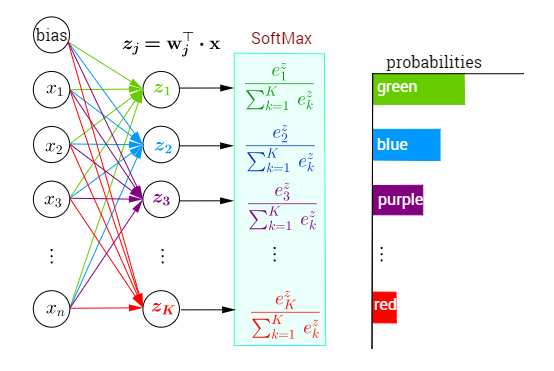
\includegraphics[width=10cm]{softmax.png}
		\caption{Multi-class classification with Neural Network using the Softmax function}
	\end{figure}

	The Softmax function for classification problems:

	\begin{equation}
		\hat{y}_j = a_j^{(L)}=\dfrac{\exp(z_j^{(L)})}{\sum_{k=1}^{d^{(L)}}\exp(z_k^{(L)})}, j=1,\dots, d^{(L)}
	\end{equation}

	\begin{equation}
		\begin{aligned}
			\dfrac{\partial a_j^{(L)}}{\partial z_j^{(L)}}&=\dfrac{\exp(z_j^{(L)})\sum_{k=1}^{d^{(L)}}\exp(z_k^{(L)}) - \exp(z_j^{(L)})\exp(z_j^{(L)})}{\Bigg(\sum_{k=1}^{d^{(L)}}\exp(z_k^{(L)})\Bigg)^2}\\&=a_j^{(L)}\Big(1- a_j^{(L)} \Big)=\hat{y}_j \Big(1 - \hat{y}_j\Big)
		\end{aligned}
	\end{equation}

	The Softmax cross entropy loss:

	\begin{equation}
		\mathcal{L}=\sum_{j=1}^{d^{(L)}}-y_j \log a_j^{(L)}+(1-y_j)\log(1-a_j^{(L)})
	\end{equation}

	Compute partial derivatives of the cross entropy loss with respect to $\bold{z}^{(L)}$:

	\begin{equation}
		\begin{aligned}
			\dfrac{\partial \mathcal{L}}{\partial a_j^{(L)}}&=-\dfrac{y_j}{a_j^{(L)}}+\dfrac{1-y_j}{1-a_j^{(L)}}\\&=\dfrac{-y_j\Big(1-a_j^{(L)}\Big)+(1-y_j)a_j^{(L)}}{a_j^{(L)}\Big(1-a_j^{(L)}\Big)}\\&=\dfrac{a_j^{(L)}-y_j}{a_j^{(L)}\Big(1-a_j^{(L)}\Big)}
		\end{aligned}
	\end{equation}

	\begin{equation}
		\begin{aligned}
			e_j^{(L)}&=\dfrac{\partial \mathcal{L}}{\partial z_j^{(L)}}\\&=\dfrac{\partial \mathcal{L}}{\partial a_j^{(L)}}\dfrac{\partial a_j^{(L)}}{\partial z_j^{(L)}}\\&=\dfrac{a_j^{(L)}-y_j}{a_j^{(L)}\Big(1-a_j^{(L)}\Big)}a_j^{(L)}\Big(1- a_j^{(L)} \Big)\\&=a_j^{(L)} - y_j =\hat{y}_j - y_j
		\end{aligned}
	\end{equation}

	\begin{equation}
		\begin{aligned}
			\bold{e}^{(L)}&=\begin{bmatrix} a_1^{(L)} - y_1 & a_2^{(L)} - y_2 & \dots & a_j^{(L)} - y_j & \dots & a_{d^{(L)}}^{(L)} - y_{d^{(L)}} \end{bmatrix}^T\\&=\begin{bmatrix} \hat{y}_1 - y_1 & \hat{y}_2 - y_2 & \dots & \hat{y}_j - y_j & \dots & \hat{y}_{d^{(L)}} - y_{d^{(L)}} \end{bmatrix}^T
		\end{aligned}
	\end{equation}

\end{frame}

\begin{frame}[allowframebreaks]{Experiment}
	The experiment uses the dataset \href{https://github.com/zalandoresearch/fashion-mnist}{Fashion Mnist} which contains 70,000 grayscale images 10 categories, showing individual articles of clothing at low resolution (28 x 28 pixels)

	The dataset was divided into two sets:
	\begin{itemize}
		\item A training set contains 60000 images and correspoding labels
  		\item A testing set contains 10000 images and correspoding labels
	\end{itemize}

	The images are displayed as 28x28 NumPy arrays, with pixel values ranging from 0 to 255. 
	
	The labels are an array of integers, ranging from 0 to 9. These correspond to the class of clothing the image represents:

	\begin{table} [h!]
		\centering
		\begin{tabular}{ || c | c  || }
		\hline
		Label & Class \\ [0.5 ex]
		\hline \hline
		0 & T-shirt/top \\ \hline
		1 & Trouser \\ \hline
		2 & Pullover \\ \hline
		3 & Dress \\ \hline
		4 & Coat \\ \hline
		5 & Sandal\\ \hline
		6 & Shirt\\ \hline 
		7 & Sneaker \\ \hline
		8 & Bag \\ \hline
		9 & Ankle boot \\ [1ex]
		\hline
		\end{tabular}
		\caption{Mapping each label to its class name}
	\end{table}

	\begin{figure}
		\centering
		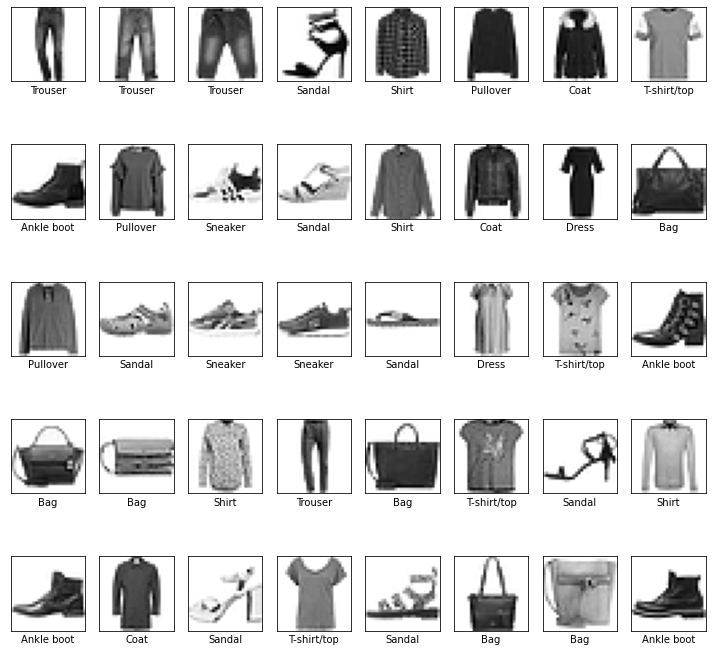
\includegraphics[width=8cm]{sample_images_with_labels.png}
		\caption{Sample of images with corresponding labels}
	\end{figure}
	The network architecture and hyperparameters:
	\begin{itemize}
		\item Each input image is flattened to a 784-d vector 
  		\item There are 2 hidden layers with 128 neurons per layer
    	\item The output layer contains 10 neuron (equals number of class)
     	\item The activation function: ReLU
      	\item Learning rates: $\lbrack 10^{-5}, 10^{-4}, 10^{-3}, 10^{-2}, 5\times10^{-2}, 10^{-1} \rbrack$
       	\item The batch size: 256
        \item The number of training epochs: 250
	\end{itemize}

	\begin{figure}
		\centering
		\resizebox{7.5cm}{!}{
			\begin{tikzpicture}[x=2.2cm,y=1.4cm]
				\message{^^JNeural network, shifted}
				\readlist\Nnod{4,5,5,3} % array of number of nodes per layer
				\readlist\Nstr{784, 128, 128, 10} % array of string number of nodes per layer
				\readlist\Cstr{\strut x,a^{(\prev)},a^{(\prev)},\hat{y}} % array of coefficient symbol per layer
				\def\yshift{0.5} % shift last node for dots
				
				\message{^^J  Layer}
				\foreachitem \N \in \Nnod{ % loop over layers
				  \def\lay{\Ncnt} % alias of index of current layer
				  \pgfmathsetmacro\prev{int(\Ncnt-1)} % number of previous layer
				  \message{\lay,}
				  \foreach \i [evaluate={\c=int(\i==\N); \y=\N/2-\i-\c*\yshift;
							   \index=(\i<\N?int(\i):"\Nstr[\lay]");
							   \x=\lay; \n=\nstyle;}] in {1,...,\N}{ % loop over nodes
					% NODES
					\node[node \n] (N\lay-\i) at (\x,\y) {$\Cstr[\lay]_{\index}$};
					
					% CONNECTIONS
					\ifnum\lay>1 % connect to previous layer
					  \foreach \j in {1,...,\Nnod[\prev]}{ % loop over nodes in previous layer
						\draw[connect,white,line width=1.2] (N\prev-\j) -- (N\lay-\i);
						\draw[connect] (N\prev-\j) -- (N\lay-\i);
						%\draw[connect] (N\prev-\j.0) -- (N\lay-\i.180); % connect to left
					  }
					\fi % else: nothing to connect first layer
					
				  }
				  \path (N\lay-\N) --++ (0,1+\yshift) node[midway,scale=1.5] {$\vdots$};
				}
				
				% LABELS
				\node[above=0.5cm,align=center,mygreen!60!black] at (N1-1.90) {784-d input};
				\node[above=0.5cm,align=center,myblue!60!black] at (N2-1.90) {128 neurons};
				\node[above=0.5cm,align=center,myblue!60!black] at (N3-1.90) {128 neurons};
				\node[above=0.5cm,align=center,myred!60!black] at (N\Nnodlen-1.90) {10 classes};
				
			\end{tikzpicture}
		}
		\caption{Neural network architecture used in experiment}
	\end{figure}
	
	\begin{figure}
		\centering
		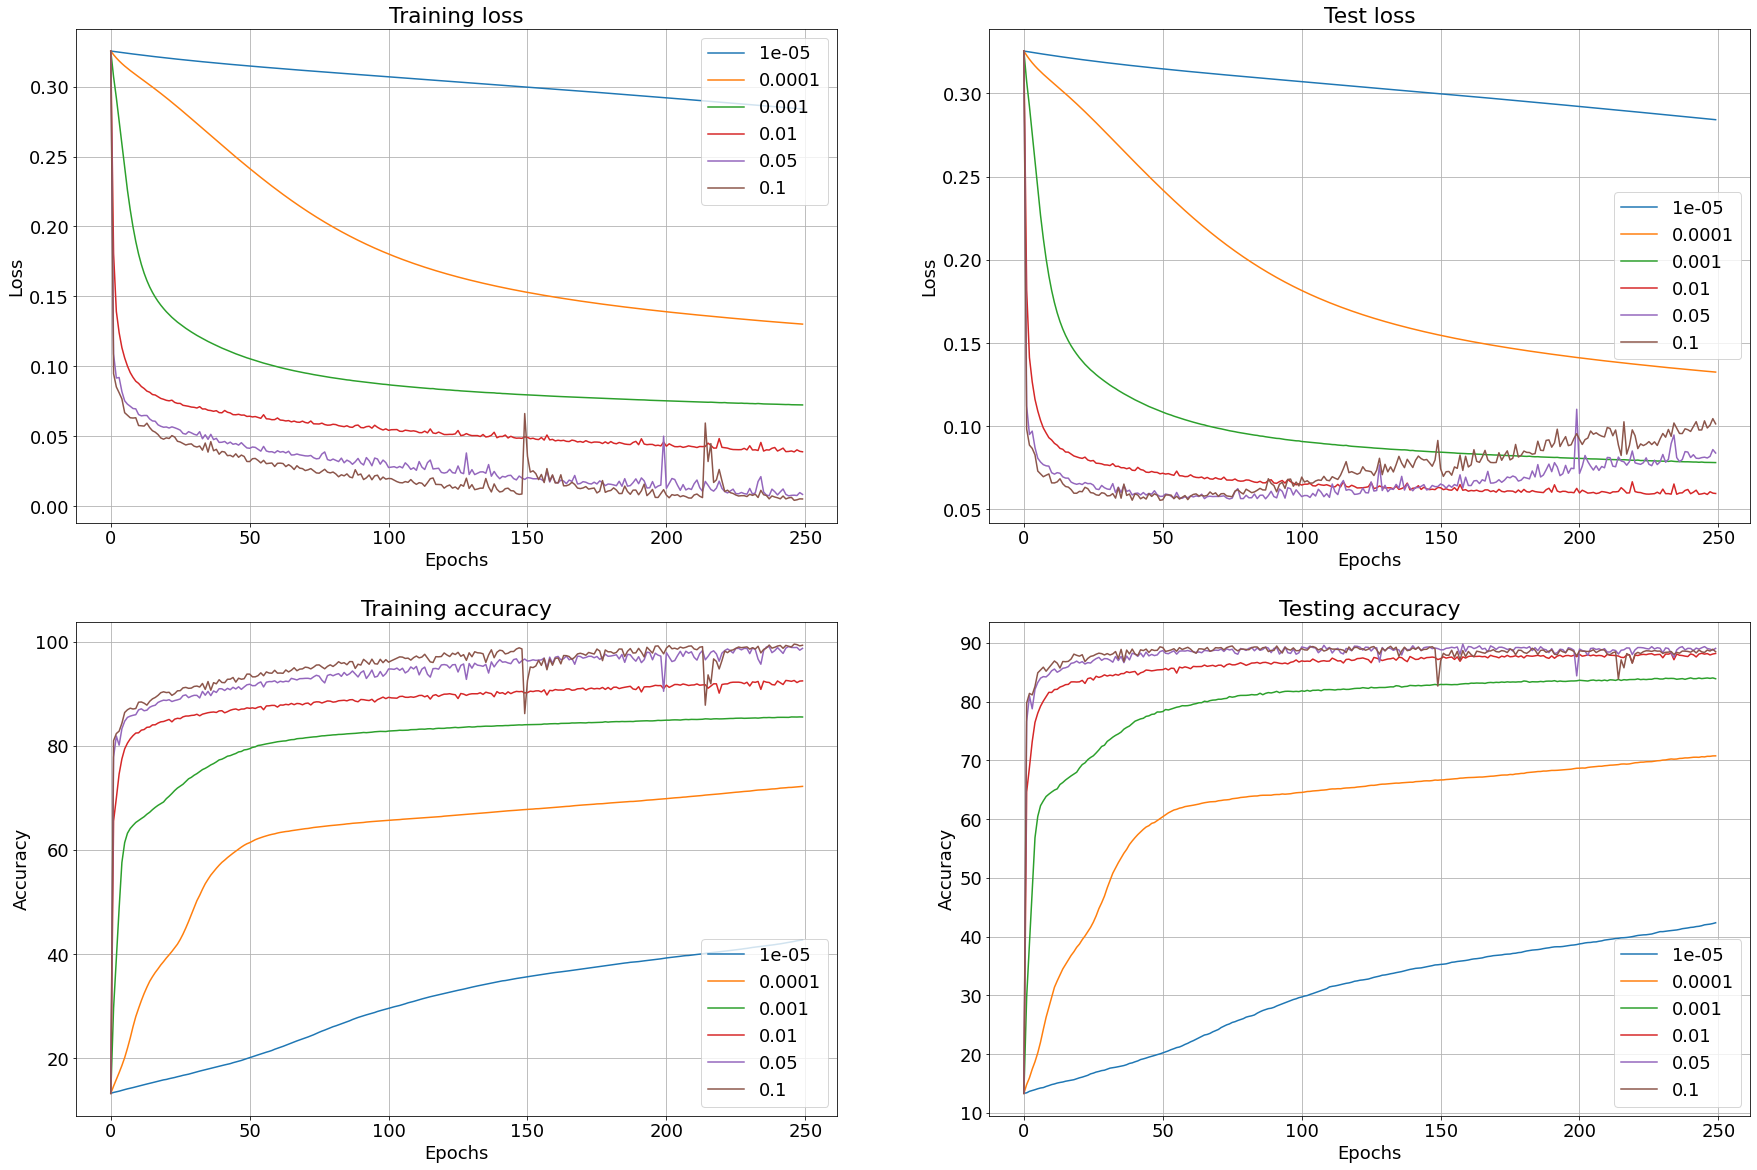
\includegraphics[width=10cm]{learning_rate_comparisons.png}
		\caption{Results with different learning rates}
	\end{figure}

	\begin{figure}
		\centering
		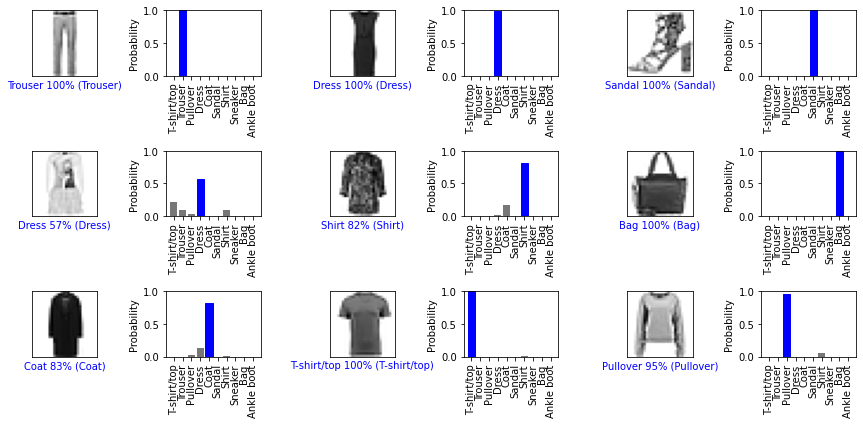
\includegraphics[width=10cm]{images_with_predictions_1.png}
		\caption{Images with corresponding predicted labels from the trained neural network}
	\end{figure}
	\begin{figure}
		\centering
		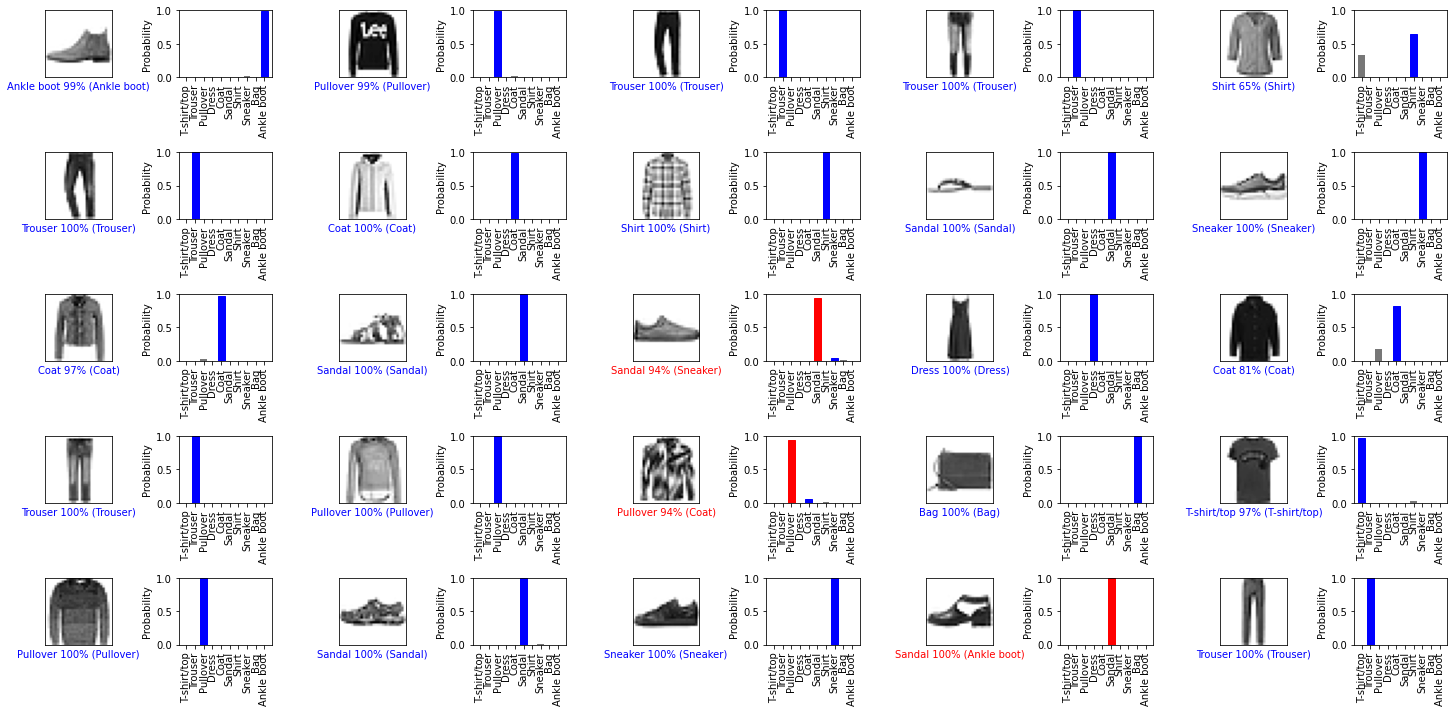
\includegraphics[width=11cm]{images_with_predictions_2.png}
		\caption{Images with corresponding predicted labels from the trained neural network}
	\end{figure}

	\begin{figure}
		\centering
		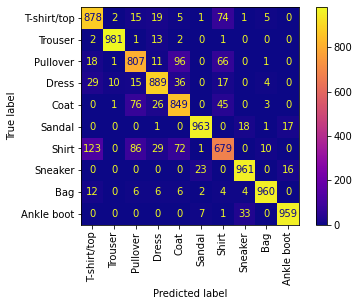
\includegraphics[width=8cm]{confusion_matrix.png}
		\caption{Confusion matrix}
	\end{figure}

	\begin{table} [h!]
		\centering
		\begin{tabular}{ || c | c | c | c | c|| }
		\hline
		Class & Precision & Recall & F1-score & Support \\ [0.5 ex]
		\hline \hline
		T-shirt/top & 0.827 & 0.878 & 0.851 & 1000 \\ \hline
		Trouser & 0.986 & 0.981 & 0.983 & 1000  \\ \hline
		Pullover & 0.802 & 0.807 & 0.805 & 1000 \\ \hline
		Dress & 0.894 & 0.889 & 0.892 & 1000 \\ \hline
		Coat & 0.796 & 0.849 & 0.822 & 1000 \\ \hline
		Sandal & 0.966 &0.963 & 0.964 & 1000\\ \hline
		Shirt & 0.766 & 0.679 & 0.720 & 1000\\ \hline 
		Sneaker & 0.945 & 0.961 & 0.953 & 1000 \\ \hline
		Bag &  0.976 & 0.960 & 0.968 & 1000 \\ \hline
		Ankle boot & 0.967 & 0.959 & 0.963 & 1000 \\ [1ex]
		\hline
		\end{tabular}
		\caption{Classification report of neural network on the testing set}
	\end{table}
\end{frame}

\begin{frame}[allowframebreaks]{Conclusion}
	\begin{itemize}
		\item Introduction about neural networks
  		\item Backpropagation in Multilayer Perceptron
    	\item Experiment on the \href{https://github.com/zalandoresearch/fashion-mnist}{Fashion Mnist} dataset
	\end{itemize}
\end{frame}

\begin{frame}[allowframebreaks]{References}
\printbibliography
\end{frame}

\end{document}